\chapter{Neural Network based Learning Agent}
\label{chap:6}
In this chapter Artificial Intelligence based agent particularly Neural Network strategy is proposed to evaluate steering of variable speed control moment gyroscope. Machine learning scheme especially reinforcement learning with combination of supervised learning is followed to train neural network \ From equations of motion and control architecture derived in it is evident that spacecraft attitude dynamics is nonlinear function of its states. Moreover singularity avoidance steering mechanism is complex and computationally expensive. Neural network are capable of approximating nonlinear functions and produce sub-optimal solution which is beneficial to reduce computational loads moreover steering is possible without matrix inversion. To design complete neural network based ACS following sections are discussed to clear some concepts. Starting with a brief introduction about machine learning types, particular interest of this thesis is focused on policy gradient method especially Proximal Policy Optimisation is discussed in detail.

\section{Machine Learning}
Machine learning is sub domain of AI is strategy to solve specific task without explicitly programming details of system. Strategy or plan is learned through available labeled data sets. Basically a black box model is approximated \ by studying large amount of input associated output, exploring unlabeled data or by enumerating inputs and outputs of black box function. Based on strategy machine learning is classified in three major parts and their a
application is shown in figure.
\begin{figure}
    \centering
    \scalebox{.5}{\begin{tikzpicture}[mindmap, grow cyclic, every node/.style=concept, concept color=gray!10, 
	level 1/.append style={font=\small,level distance=5cm,sibling angle=120},
	level 2/.append style={font=\tiny,level distance=3cm,sibling angle=70},
	level 3/.append style={font=\tiny,font=\tiny,level distance=3cm,sibling angle=30},]


\node{Machine Learning}
child { node {Supervised Learning}
    child { node {Regression}
        child { node {Decision Tree}}
        child { node {Linear Regression}}
        child { node {Logistic Regression}} }
    child { node {Classification}
        child { node {Support Vector Machine}}
        child { node {Navie Bayes}}
        child { node {K-Nearest Neighbor}} }
    }
child { node {Unsupervised Learning}
    child { node {Clustering}
        child { node {K-Means}}
        child { node {Mean Shift}}
        child { node {K-Medoids}} }
    child { node {Dimensionality Reduction}
        child { node {Principle Component Analysis (PCA)}}
        child { node {Feature Selection}}
        child { node {Linear Discriminant Analysis (LDA)}} }
    }
child { node {Reinforcement Learning}
        child { node {Real time decisions}}
        child { node {Robot Navigation}}
        child { node {Learning Task}}
        child { node {Skill Acquisition}}
        child { node {Game AI}}
    };

\end{tikzpicture}}
    \caption{Machine Learning Classifications}
    \label{fig:ML_Mindmap}
\end{figure}
\subsection{Supervised Learning}
In this strategy labeled output for particular inputs are known and agent learns relation from input and output mostly used in predictive analysis. Explicitly defined labels are needed hence the name. Model predicts output based on current input and later compare it with labeled output. Two types of supervised learning are classification with categorical output and reparation with numerical output such as fitting a curve. In this thesis supervised learning is used to partially learn strategy from data set produced using steering law discussed in previous chapter in order to reduce training time.

\subsection{Unsupervised Learning}
Machine learns by exploring large chunk of unlabeled data set. Clustering and dimensionality reduction are two sub-classes of unsupervised learning. In this case information is retrieved from data set with keeping simpler and spars representation than original data, can be used to discover pasterns in given data-set. In pattern recognition similar data samples are clustered together.

\newacronym{mdp}{MDP}{Markov Decision Processes}
\subsection{Reinforcement Learning}
Reinforcement learning is a close loop problem where agent takes action, each action is associated with reward or penalty, and based on outcome agent tries to maximize reward or minimize the penalty by exploring in to environment or exploiting past experiences through trial and error along with received feedback. \autoref{fig:ai_agent_env_mdp} shows architecture of agent-environment interaction in \acrlong{mdp}.\cite{russell2010artificial}

\begin{figure}[H]
    \centering

\tikzset{
  frame/.style={
    rectangle, draw,
    text width=6em, text centered,
    minimum height=4em,drop shadow,fill=white,
    rounded corners,
  },
  line/.style={
    draw, -{Latex},rounded corners=0.5mm,
  }
}
\begin{tikzpicture}[font=\small\sffamily\bfseries,very thick,node distance = 4cm]
\node [frame] (agent) {Agent};
\node [frame, below=1.2cm of agent] (environment) {Environment};
\draw[line] (agent) -- ++ (3.5,0) |- (environment)
node[right,pos=0.25,align=left] {action\\ $a_t$};
\coordinate[left=8mm of environment] (P);
\coordinate[above=3mm of environment.west] (ENW);
\coordinate[below=3mm of environment.west] (ESW);
\coordinate[above=3mm of agent.west] (ANW);
\coordinate[below=3mm of agent.west] (ASW);
\draw[thin,dashed] (P|-environment.north) -- (P|-environment.south);
\draw[line] (ESW) -- (P |- ESW)
node[midway,above]{$s_{i+1}$};
\draw[line,thick] (ENW) -- (P |- ENW)
node[midway,above]{$a_{i+1}$};
\draw[line] (P |- ESW) -- ++ (-1.4,0) |- (ANW)
node[left, pos=0.25, align=right] {state\\ $s_t$};
\draw[line,thick] (P |- ENW) -- ++ (-0.8,0) |- (ASW)
node[right,pos=0.25,align=left] {reward\\ $r_t$};
\end{tikzpicture}

    \caption{The agent-environment interaction in  interaction in a Markov Decision Process. \cite{sutton2018reinforcement}}
    \label{fig:ai_agent_env_mdp}
\end{figure}

\noindent\textbf{Agent} is any entity that perceives environment using sensors and acts on it using actuators. A rational agent should take appropriate actions based on strategy to reach goal. Success of agent is determined by performance measure.
Agent function that maps precept history to action is given as:
\begin{equation}
    f: \mathcal{P}^*\longrightarrow \mathcal{A}
\end{equation}
\textbf{Environment} is a real situation or simulated plant dynamics and may have properties such fully or partially observable, deterministic or stochastic, discrete or continuous.
\textbf{Perceptions} are observed states $s\in \mathcal{S}$ in the environment through sensors whereas \textbf{actions} $a\in \mathcal{A}$ are performed by agent through actuators
Agent at state $s$ inside environment, chooses one action $a$ among many choices in order to evolve its state and evolution is determined by state transition probability. For each action, environment provides reward $r \in \mathcal{R}$ as feedback. The \acrfull{mdp} consists of set of states $\mathcal{S}$, set of actions $\mathcal{A}$, transition probability function $P$ reward function $R$, discounting factor for future rewards $\gamma$
\begin{equation*}
    \mathcal{M} = \langle \mathcal{S}, \mathcal{A}, P, R, \gamma \rangle
\end{equation*}
\noindent A \textbf{Policy} $\pi(s)$  is, therefore, a strategy that an agent uses in pursuit of goals.\cite{russell2010artificial} Policy determines actions that has to be taken by agent at state $s$. Policy can be deterministic: $\pi(s)=a$ or stochastic:$\pi(a \vert s) = \mathbb{P}_\pi [A=a \vert S=s]$

Each state is associated with a \textbf{Value} $V(s)$ function which is probability of future rewards than can be received by acting on policy at given state. With future reward as total some of rewards going forward from time t noted as $G_t$
\begin{equation}
    G_t = R_{t+1} + \gamma R_{t+2} + \dots = \sum_{k=0}^{\infty} \gamma^k R_{t+k+1}
\end{equation}
Here discount factor $\gamma \in [0,1]$ is introduced to  penalize the future rewards since propagation of uncertainty becomes larger for long time. The state value is expected return at given state:
\begin{equation}
    V_{\pi}(s) = \mathbb{E}_{\pi}[G_t \vert S_t = s] = \sum_{a \in \mathcal{A}} Q_{\pi}(s, a) \pi(a \vert s)
\end{equation}
Where, action-value of state action pair
\begin{equation}
Q_{\pi}(s, a) = \mathbb{E}_{\pi}[G_t \vert S_t = s, A_t = a]    
\end{equation}
\textbf{Advantage function} $A(s,a)$ is difference between state-value and action value, it asses quality of selected action with respect to certain state.  
\begin{equation}
    A_{\pi}(s, a) = Q_{\pi}(s, a) - V_{\pi}(s)
\end{equation}
An optimum value function that produces maximum returns is
\begin{equation}
    V_{*}(s) = \max_{\pi} V_{\pi}(s),
Q_{*}(s, a) = \max_{\pi} Q_{\pi}(s, a)
\end{equation}
and the policy that achieves optimum value function is optimal policy given as
\begin{equation}
    \pi_{*} = \arg\max_{\pi} V_{\pi}(s),
\pi_{*} = \arg\max_{\pi} Q_{\pi}(s, a)
\end{equation}
The agent-environment interaction is produces series of state, action and reward each time step evolved from $t=0,1,2,\dots,T$. Hence, evolution is sequence state $S_t \in \mathcal{S}$, action $A_t \in \mathcal{A}(s)$ and rewards $R_{t+1} \in \mathcal{R}$ taken at each time $t$ to end of an episode at terminal time $T$.
\acrlong{mdp} shown in \autoref{fig:ai_agent_env_mdp} gives rise to sequence:
\begin{equation*}
    S_0, A_0, R_1,S_1, A_1, R_2, \dots S_{T}, A_{T}, R_{T+1},
\end{equation*}
The model is function that describes environment with associated transition probability $P$ and reward function $R$. Evaluation from state $s$ to next state $s'$ fro action $a$ and associated reward $r$ is transition step and represented as tuple $(s,a,s',r)$. The probability of transition ${\displaystyle s\xrightarrow[a]{} s'}$ is given as
\begin{equation}
P(s',r|s,a)=\mathbb{P} [S_{t+1} =s',R_{t+1} =r|S_{t} =s,A_{t} =a]
\end{equation}
state transition matrix as function of $\displaystyle P(s',r|s,a)$:
\begin{equation}
P^{a}_{ss'} =P(s'|s,a)=\mathbb{P} [S_{t+1} =s'|S_{t} =s,A_{t} =a]=\sum _{r\in \mathcal{R}} P(s',r|s,a)
\end{equation}
and reward function that predicts next reward upon action is
\begin{equation*}
R(s,a)=\mathbb{E} [R_{t+1} |S_{t} =s,A_{t} =a]=\sum _{r\in \mathcal{R}} r\sum _{s'\in \mathcal{S}} P(s',r|s,a)
\end{equation*}


In MDP future only depends on current state and does not have effects of history.
\begin{equation}
\mathbb{P} [S_{t+1} |S_{t} ]=\mathbb{P} [S_{t+1} |S_{1} ,\dotsc ,S_{t} ]
\end{equation}

Decomposition of value function in to immediate reward and the discounted future values using Bellman Equations as
\begin{equation}
\begin{aligned}
V(s) & =\mathbb{E} [G_{t} |S_{t} =s]\\
 & =\mathbb{E} [R_{t+1} +\gamma R_{t+2} +\gamma ^{2} R_{t+3} +\dotsc |S_{t} =s]\\
 & =\mathbb{E} [R_{t+1} +\gamma (R_{t+2} +\gamma R_{t+3} +\dotsc )|S_{t} =s]\\
 & =\mathbb{E} [R_{t+1} +\gamma G_{t+1} |S_{t} =s]\\
 & =\mathbb{E} [R_{t+1} +\gamma V(S_{t+1} )|S_{t} =s]
\end{aligned}
\end{equation}
and action value also referred as Q value is 
\begin{equation}
\begin{aligned}
Q(s,a) & =\mathbb{E} [R_{t+1} +\gamma V(S_{t+1} )\mid S_{t} =s,A_{t} =a]\\
 & =\mathbb{E} [R_{t+1} +\gamma \mathbb{E}_{a\sim \pi } Q(S_{t+1} ,a)\mid S_{t} =s,A_{t} =a]
\end{aligned}
\end{equation}


\section{Policy Gradient Methods}
In order to solve RL problem that is to find optimal strategy with which agent achieves optimal rewards. Policy Gradient Method \cite{Grondman2012} learns with parametrized function of $\displaystyle \theta ,\pi _{\theta } (a|s)$. The reward value depends on the policy and learning is done through optimizing $\displaystyle \theta $ for best rewards. The reward function is defined as:
\begin{equation}
J(\theta )=\sum _{s\in \mathcal{S}} d^{\pi } (s)V^{\pi } (s)=\sum _{s\in \mathcal{S}} d^{\pi } (s)\sum _{a\in \mathcal{A}} \pi _{\theta } (a|s)Q^{\pi } (s,a)
\end{equation}
here \ $\displaystyle d^{\pi }$ is the stationary distribution of Markov chain for $\displaystyle \pi _{\theta }$. The idea is for by exploring states of

Markov chain for long period of time, probability of conversing to one state becomes constant and known as stationary probability for $\displaystyle \pi _{\theta }$. Starting from initial state $\displaystyle s_{0}$ up to state $\displaystyle s_{t}$ with using policy $\displaystyle \pi _{\theta }$ the stationary distribution \ $\displaystyle d^{\pi }$ is given as:
\begin{equation}
d^{\pi } (s)=\lim _{t\rightarrow \infty } P(s_{t} =s|s_{0} ,\pi _{\theta } )
\end{equation}


Now with using gradient ascent search for best $\displaystyle \theta $ that gives maximum rewards.

\subsection{Policy Gradient Theorem}
Consider the $\displaystyle \theta $ with $\displaystyle k$ dimensions is to be optimized, numerical gradient of $\displaystyle \theta $ can be found with \ introducing small perturbation $\displaystyle \epsilon $ 
\begin{equation}
\frac{\partial J(\theta )}{\partial \theta _{k}} \approx \frac{J(\theta +\epsilon u_{k} )-J(\theta )}{\epsilon }
\end{equation}
 and for analytical gradient of \ $\displaystyle J(\theta )$
\begin{equation}
\begin{aligned}
J(\theta ) & =\sum _{s\in \mathcal{S}} d(s)\sum _{a\in \mathcal{A}} \pi (a|s,\theta )Q_{\pi } (s,a)\\
\nabla J(\theta ) & =\sum _{s\in \mathcal{S}} d(s)\sum _{a\in \mathcal{A}} \nabla \pi (a|s,\theta )Q_{\pi } (s,a)\\
 & =\sum _{s\in \mathcal{S}} d(s)\sum _{a\in \mathcal{A}} \pi (a|s,\theta )\frac{\nabla \pi (a|s,\theta )}{\pi (a|s,\theta )} Q_{\pi } (s,a)\\
 & =\sum _{s\in \mathcal{S}} d(s)\sum _{a\in \mathcal{A}} \pi (a|s,\theta )\nabla \ln \pi (a|s,\theta )Q_{\pi } (s,a)\\
 & =\mathbb{E}_{\pi _{\theta }} [\nabla \ln \pi (a|s,\theta )Q_{\pi } (s,a)]
\end{aligned}
\end{equation}
and finally, we get policy gradient theorem as
\begin{equation}
\nabla J(\theta )=\mathbb{E}_{\pi _{\theta }} [\nabla \ln \pi (a|s,\theta )Q_{\pi } (s,a)]
\end{equation}
Since probabilities of each actions are not computed,policy gradient methods are suitable for continuous action space.

\subsection{Proximal Policy Optimization (PPO)}
Proposed by John et. al. PPO\cite{schulman2017proximal} which optimizes a clipped/surrogate objective function using stochastic gradient ascent. In this method multiple epochs of mini batch updates are used instead of one update per batch. Let consider probability ratio of old and new policies as:
\begin{equation}
r(\theta )=\frac{\pi _{\theta } (a|s)}{\pi _{\theta _{\text{old}}} (a|s)}
\end{equation}

\noindent then objective function of TRPO\footnote{Trust Region Policy Optimization\cite{schulman2015trust} avoids parameter updates that change the policy rapidly} is reduced to
\begin{equation}
J^{TRPO} (\theta )=\mathbb{E}[ r(\theta )\hat{A}_{\theta _{old}} (s,a)]
\end{equation}
if distance between $\displaystyle \theta _{old}$ and $\displaystyle \theta $ is not limited, extremely large parameter updates will be made to optimize $\displaystyle J^{TRPO}( \theta )$, leading to instability. In PPO $\displaystyle r( \theta )$ is bounded close to $\displaystyle 1\pm \epsilon $, here $\displaystyle \epsilon $ is hyperparameter and minimum of either same objective or clipped objective is selected.
\begin{equation}
J^{CLIP} (\theta )=\mathbb{E} [\min (r(\theta )\hat{A}_{\theta _{old}} (s,a),clip(r(\theta ),1-\epsilon ,1+\epsilon )\hat{A}_{\theta _{old}} (s,a))]
\end{equation}
ratio $\displaystyle r( \theta )$ is clipped between $\displaystyle 1-\epsilon $ and $\displaystyle 1+\epsilon $ as shown in \autoref{fig:ppo_cliped} surrogate $J^{CLIP}(\theta)$ as function of probability ratio $r$ for one step starting from $r=1$. since ratio is clipped and does not vary rapidly large policy updates are skipped hence increasing stability. \autoref{algo_PPO_AC} is actor critic style parallel implementation of PPO.

\begin{figure}[H]
    \centering
    

\tikzset{every picture/.style={line width=0.75pt}} %set default line width to 0.75pt        

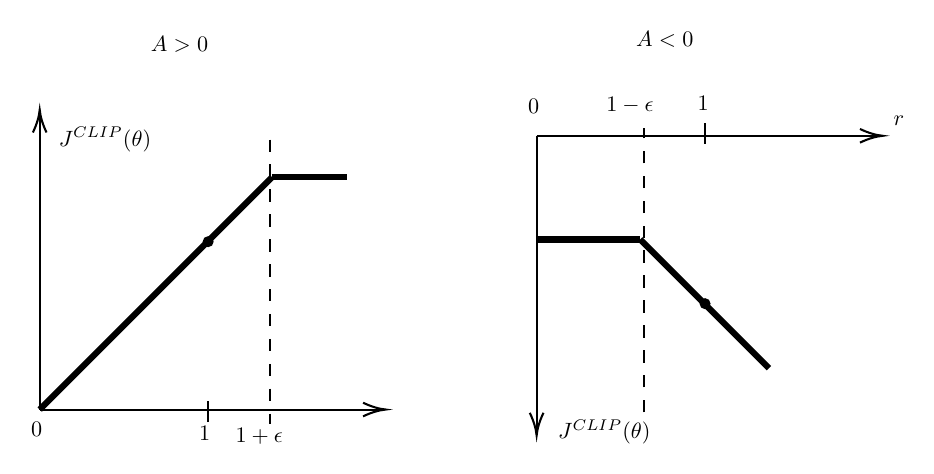
\begin{tikzpicture}[x=0.75pt,y=0.75pt,yscale=-1,xscale=1]
%uncomment if require: \path (0,283); %set diagram left start at 0, and has height of 283

%Straight Lines [id:da07428987415964317] 
\draw    (60.04,246.51) -- (60.04,104.1) ;
\draw [shift={(60.04,102.1)}, rotate = 450] [color={rgb, 255:red, 0; green, 0; blue, 0 }  ][line width=0.75]    (10.93,-3.29) .. controls (6.95,-1.4) and (3.31,-0.3) .. (0,0) .. controls (3.31,0.3) and (6.95,1.4) .. (10.93,3.29)   ;
%Straight Lines [id:da42162293191171707] 
\draw    (60.04,246.51) -- (224.76,246.51) ;
\draw [shift={(226.76,246.51)}, rotate = 180] [color={rgb, 255:red, 0; green, 0; blue, 0 }  ][line width=0.75]    (10.93,-3.29) .. controls (6.95,-1.4) and (3.31,-0.3) .. (0,0) .. controls (3.31,0.3) and (6.95,1.4) .. (10.93,3.29)   ;
%Straight Lines [id:da46857481861880057] 
\draw  [dash pattern={on 4.5pt off 4.5pt}]  (170.93,116.45) -- (170.93,253.43) ;
%Straight Lines [id:da5916594745882346] 
\draw [line width=2.25]    (60.04,246.51) -- (171.98,134.58) ;
%Straight Lines [id:da20769803027157696] 
\draw [line width=2.25]    (171.98,134.58) -- (208.01,134.58) ;
%Shape: Ellipse [id:dp9944817970164661] 
\draw  [fill={rgb, 255:red, 0; green, 0; blue, 0 }  ,fill opacity=1 ] (139.07,165.63) .. controls (139.07,164.46) and (140.02,163.51) .. (141.19,163.51) .. controls (142.36,163.51) and (143.31,164.46) .. (143.31,165.63) .. controls (143.31,166.8) and (142.36,167.75) .. (141.19,167.75) .. controls (140.02,167.75) and (139.07,166.8) .. (139.07,165.63) -- cycle ;
%Straight Lines [id:da631388526485618] 
\draw    (141.19,252.63) -- (141.19,242.51) ;
%Straight Lines [id:da5700736740675836] 
\draw    (299.45,114.62) -- (299.45,257.03) ;
\draw [shift={(299.45,259.03)}, rotate = 270] [color={rgb, 255:red, 0; green, 0; blue, 0 }  ][line width=0.75]    (10.93,-3.29) .. controls (6.95,-1.4) and (3.31,-0.3) .. (0,0) .. controls (3.31,0.3) and (6.95,1.4) .. (10.93,3.29)   ;
%Straight Lines [id:da4383859714024194] 
\draw    (299.45,114.62) -- (464.17,114.62) ;
\draw [shift={(466.17,114.62)}, rotate = 540] [color={rgb, 255:red, 0; green, 0; blue, 0 }  ][line width=0.75]    (10.93,-3.29) .. controls (6.95,-1.4) and (3.31,-0.3) .. (0,0) .. controls (3.31,0.3) and (6.95,1.4) .. (10.93,3.29)   ;
%Straight Lines [id:da15252831399229727] 
\draw [line width=2.25]    (349.38,164.55) -- (411.38,226.55) ;
%Straight Lines [id:da20676916509391385] 
\draw [line width=2.25]    (299.29,164.55) -- (349.38,164.55) ;
%Shape: Ellipse [id:dp5844715267834208] 
\draw  [fill={rgb, 255:red, 0; green, 0; blue, 0 }  ,fill opacity=1 ] (378.47,195.5) .. controls (378.47,196.67) and (379.42,197.62) .. (380.59,197.62) .. controls (381.77,197.62) and (382.72,196.67) .. (382.72,195.5) .. controls (382.72,194.33) and (381.77,193.38) .. (380.59,193.38) .. controls (379.42,193.38) and (378.47,194.33) .. (378.47,195.5) -- cycle ;
%Straight Lines [id:da16120535517562784] 
\draw    (380.59,108.5) -- (380.59,118.62) ;
%Straight Lines [id:da12247292832159551] 
\draw  [dash pattern={on 4.5pt off 4.5pt}]  (350.97,247.88) -- (350.97,110.91) ;

% Text Node
\draw (470.29,103.87) node [anchor=north west][inner sep=0.75pt]  [xscale=0.8,yscale=0.8]  {$r$};
% Text Node
\draw (68.02,109.38) node [anchor=north west][inner sep=0.75pt]  [xscale=0.8,yscale=0.8]  {$J^{CLIP}( \theta )$};
% Text Node
\draw (135.61,253.59) node [anchor=north west][inner sep=0.75pt]  [xscale=0.8,yscale=0.8]  {$1$};
% Text Node
\draw (153.24,254.39) node [anchor=north west][inner sep=0.75pt]  [xscale=0.8,yscale=0.8]  {$1+\epsilon $};
% Text Node
\draw (112.41,65.43) node [anchor=north west][inner sep=0.75pt]  [xscale=0.8,yscale=0.8]  {$A >0$};
% Text Node
\draw (308.62,250.38) node [anchor=north west][inner sep=0.75pt]  [xscale=0.8,yscale=0.8]  {$J^{CLIP}( \theta )$};
% Text Node
\draw (375.82,94.26) node [anchor=north west][inner sep=0.75pt]  [xscale=0.8,yscale=0.8]  {$1$};
% Text Node
\draw (331.89,95.06) node [anchor=north west][inner sep=0.75pt]  [xscale=0.8,yscale=0.8]  {$1-\epsilon $};
% Text Node
\draw (294.15,95.86) node [anchor=north west][inner sep=0.75pt]  [xscale=0.8,yscale=0.8]  {$0$};
% Text Node
\draw (54.74,251.19) node [anchor=north west][inner sep=0.75pt]  [xscale=0.8,yscale=0.8]  {$0$};
% Text Node
\draw (346.2,63.03) node [anchor=north west][inner sep=0.75pt]  [xscale=0.8,yscale=0.8]  {$A< 0$};


\end{tikzpicture}    \caption{Surrogate $J^{CLIP}(\theta)$as function of probability ratio for positive (left) and negative (right) advantage, figure reconstructed from original paper. \cite{schulman2017proximal}}
    \label{fig:ppo_cliped}
\end{figure}


\begin{algorithm}[H]
\SetAlgoLined
\KwResult{Write here the result }
\For{iteration=$1,2,\dots$} {
\For{actor=$1,2,\dots,N$} {
Run policy $\displaystyle \pi_{\theta_{old}}$ in environment for $T$ time steps.\\
Compute advantage estimates $\hat{A}_1,\dots,\hat{A}_T$
}
Optimize surrogate $L$ wrt $\theta$, with $K$ epochs and minibatch size $M \leq NT$ \\
$\theta_{old} \xleftarrow[]{} \theta$
}
 \caption{PPO,Actor-Critic Style}
    \label{algo_PPO_AC}
\end{algorithm}
\section{Neural Network}
Neural networks were first introduced  in 1944 by Warren McCullough and Walter Pitts. Inspired by human brain neural networks are large graphs made up of densely connected processing nodes. Theses processing nodes are referred as neurons, It may take multiple inputs and produce one output. Each input $x_i$ is associated with some weight $w_i$, neuron produces weighted some of inputs adds bias to it and squeezes the results with pre-selected activation function. As shown in \autoref{fig:neuron} neuron functions as
\begin{equation}
    y_{out} = f(b+\sum ^{n}_{i=1} x_i,w_i)
\end{equation}
\begin{figure}[H]
    \centering
    
    \begin{tikzpicture}[
    % define styles    
    init/.style={ 
         draw, 
         circle, 
         inner sep=2pt,
         font=\Huge,
         join = by -latex
    },
    squa/.style={ 
        font=\Large,
        join = by -latex
    }
]
% Top chain x1 to w1
\begin{scope}[start chain=1]
    \node[on chain=1] at (0,1.5cm)  (x1) {$x_1$};
    \node[on chain=1,join=by o-latex] (w1) {$w_1$};
\end{scope}
% Middle chain x2 to output
\begin{scope}[start chain=2]
    \node[on chain=2] (x2) {$x_2$};
    \node[on chain=2,join=by o-latex](w2) {$w_2$};
    \node[on chain=2,init] (sigma) {$\displaystyle\Sigma$};
    \node[on chain=2,squa,label=above:{\parbox{2cm}{\centering Activation\\ function}}]   {$f$};
    \node[on chain=2,squa,label=above:Output,join=by -latex] {$y_{out}$};
\end{scope}
% Bottom chain x3 to w3
\begin{scope}[start chain=3]
    \node[on chain=3] at (0,-1.5cm) 
    (x3) {$x_n$};
    \node[on chain=3,label=below:Weights,join=by o-latex]
    (w3) {$w_n$};
\end{scope}
% Bias
\node[label=above:\parbox{2cm}{\centering Bias \\ $b$}] at (sigma|-w1) (b) {};
% Arrows joining w1, w3 and b to sigma
\draw[-latex] (w1) -- (sigma);
\draw[-latex] (w3) -- (sigma);
\draw[o-latex] (b) -- (sigma);

\draw[dotted](w2) -- (w3);

% left hand side brace
\draw[decorate,decoration={brace,mirror}] (x1.north west) -- node[left=10pt] {Inputs} (x3.south west);

\end{tikzpicture}
    \caption{Components of individual Neuron.The activation function is denoted by $f$ and applied on the weighted sum of inputs with added bias}
    \label{fig:neuron}
\end{figure}
\noindent Activation function is basically squeezing of weighted sum in to some allowable values, sometimes activation can be just an trigger which occurs after reaching decided threshold. Shapes of commonly used activation functions are shown in \autoref{fig:act_func}. Apart from its shape most important property of activation function is its derivative which has crucial role for training a neural network. Few commonly used activation functions are mentioned in \autoref{tbl_act_func}

\begin{figure}[H]
\centering
 \begin{subfigure}[t]{0.45\columnwidth}
 \centering
         
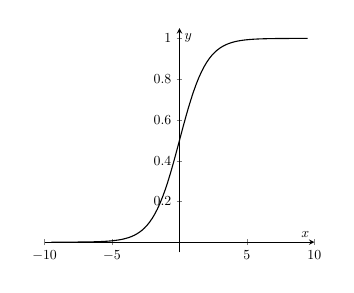
\begin{tikzpicture}[scale = 0.5]
\begin{axis}[
    axis lines=middle,
    xmax=10,
    xmin=-10,
    ymin=-0.05,
    ymax=1.05,
    xlabel={$x$},
    ylabel={$y$}
]
\addplot [domain=-9.5:9.5, samples=100,
          thick, black] {1/(1+exp(-x)};
\end{axis}
\end{tikzpicture}

 \caption{Sigmoid}
 \label{fig:act_sigmoid}
 \end{subfigure}
~ 
 \begin{subfigure}[t]{0.45\columnwidth}
 \centering

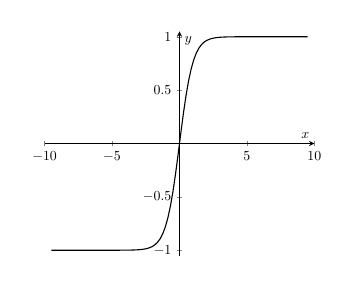
\begin{tikzpicture}[scale = 0.5]
\begin{axis}[
    axis lines=middle,
    xmax=10,
    xmin=-10,
    ymin=-1.05,
    ymax=1.05,
    xlabel={$x$},
    ylabel={$y$}]
\addplot [domain=-9.5:9.5, samples=100,
     thick, black] {(exp(x) - exp(-x))/(exp(x) + exp(-x))};
\end{axis}
\end{tikzpicture}

 \caption{tanh}
 \label{fig:act_tanh}
 \end{subfigure}
~ 
 \begin{subfigure}[t]{0.45\columnwidth}
 \centering

\begin{tikzpicture}[scale = 0.5]
\begin{axis}[
    axis lines=middle,
    xmax=6,
    xmin=-6,
    ymin=-0.05,
    ymax=5.05,
    xlabel={$x$},
    ylabel={$y$}]
\addplot [domain=-5.5:5.5, samples=100, thick, black] {max(0, x)};
\end{axis}
\end{tikzpicture}

 \caption{ReLu}
 \label{fig:act_relu}
 \end{subfigure}
~ 
 \begin{subfigure}[t]{0.45\columnwidth}
 \centering
\begin{tikzpicture}[scale = 0.5]
\begin{axis}[
    axis lines=middle,
    xmax=6,
    xmin=-6,
    ymin=-1.05,
    ymax=5.05,
    xlabel={$x$},
    ylabel={$y$}]
\addplot [domain=-5.5:5.5, samples=100,
          thick, black] {max(0.1 * x, x)};
\end{axis}
\end{tikzpicture}
\caption{Leaky ReLu}
\label{fig:act_leackrelu}
     \end{subfigure}
     
\caption{Commonly used activation functions}
\label{fig:act_func}
\end{figure}


\begin{table}[H]
        \centering
\begin{tabular}{p{0.3\textwidth}|p{0.3\textwidth}|p{0.3\textwidth}}
\toprule
 Activation Function & Function $\displaystyle f(z)$ & Derivative $\displaystyle f'(z)$ \\
\midrule
 Sigmoid & {\small $\displaystyle f(z)=\frac{1}{1+e^{-z}}$} & {\small $\displaystyle f'( z) \ =\ f( z) \ \cdotp ( 1\ -\ f( z))$} \\
\hline 
 Tanh & {\small $\displaystyle f(z)=\frac{e^{z} -e^{-z}}{e^{z} +e^{-z}}$} & {\small $\displaystyle f'(z)=1-\tanh (z)^{2}$} \\
\hline 
 Linear & {\small $\displaystyle f( z) =z\alpha $} & {\small $\displaystyle f'( z) =\alpha $} \\
\hline 
 Exponential Linear Unit (ELU) & {\small $\displaystyle f( z) =\begin{cases}
z & z >0\\
\alpha \left( e^{z} -1\right) & z\leq 0
\end{cases}$} & {\small $\displaystyle f'( z) =\begin{cases}
1 & z >0\\
\alpha e^{z} & z\leq 0
\end{cases}$} \\
\hline 
 Rectified Linear Units (ReLU) & {\small $\displaystyle f( z) =\begin{cases}
z & z >0\\
0 & ,z\leq 0
\end{cases}$} & {\small $\displaystyle f'( z) =\begin{cases}
z & z >0\\
0 & z\leq 0
\end{cases}$} \\
\hline 
 LeakyRelu & {\small $\displaystyle f( z) =\begin{cases}
z & z >0\\
\alpha z & z\leq 0
\end{cases}$} & {\small $\displaystyle f'( z) =\begin{cases}
z & z >0\\
\alpha  & z\leq 0
\end{cases}$} \\
\hline 
 Arctan & {\small $\displaystyle f( z) =\tan^{-1}( z)$} & {\small $\displaystyle f'( z) =\frac{1}{1+z^{2}}$} \\
\hline 
 Swish & {\small $\displaystyle f(z)=\frac{z}{1+e^{-z}}$} & {\small $\displaystyle f'(z)=\frac{f( z)( 1-f( z))}{1+e^{-z}}$} \\
\hline 
 Soft Plus & {\small $\displaystyle f(z)=\ln\left( 1+e^{z}\right)$} & {\small $\displaystyle f'(z)=\frac{1}{1+e^{-z}}$} \\

\bottomrule
\end{tabular}
\caption{Commonly used activation functions and their derivative}
\label{tbl_act_func}
\end{table}

\newacronym{mlp}{MLP}{Multi Layer Perceptron}
\subsection{Multi Layer Perceptron policy}
\acrlong{mlp} is a complex network of perceptrons connected based on various architectures. Most common method is feed forward neural network. Neurons are grouped in a single stage called a layers. Every unit in a layer is connected to all units of previous layers. Three distinct layers are Input, Hidden and Output. Data enters from input and passes thorough hidden layers finally emitted from output layer. Hidden layers are not accessible to external world hence the name. Shallow neural network has one hidden layer as opposed to Deep neural networks, which may have multiple hidden layers, an example shown in \autoref{fig:mlp}. With properly chosen weights, Neural network can approximate any nonlinear function. Process of finding weights is called training an iterative process where data is passed from input layer and based on error between evaluated and expected output weights are updated in backward direction layer by layer, process referred as propagation.
\begin{figure}
    \centering
    \scalebox{0.65}{

\begin{tikzpicture}[x=1.5cm, y=1.5cm, >=stealth]
\tikzset{%
  every neuron/.style={
    circle,
    draw,
    minimum size=1cm
  },
  neuron missing/.style={
    draw=none, 
    scale=2,
    text height=0.333cm,
    execute at begin node=\color{black}$\vdots$
  },
}
% Input
\foreach \m/\l [count=\y] in {1,2,missing,3}
  \node [every neuron/.try, neuron \m/.try] (input-\m) at (0, 3-\y*1.2) {};
% h1 1
\foreach \m [count=\y] in {1,2,3,missing,4}
  \node [every neuron/.try, neuron \m/.try ] (h1-\m) at (2, 3.6-\y*1.2) {};
% h1 2
\foreach \m [count=\y] in {1,2,3,missing,4}
  \node [every neuron/.try, neuron \m/.try ] (h2-\m) at (4, 3.6-\y*1.2) {};
% h1 3
\foreach \m [count=\y] in {1,2,3,missing,4}
  \node [every neuron/.try, neuron \m/.try ] (h3-\m) at (6, 3.6-\y*1.2) {};

% h1 4
\foreach \m [count=\y] in {1,2,3,missing,4}
  \node [every neuron/.try, neuron \m/.try ] (h4-\m) at (8, 3.6-\y*1.2) {};

% Output
\foreach \m [count=\y] in {1,2,missing,3}
  \node [every neuron/.try, neuron \m/.try ] (output-\m) at (10,3-\y*1.2) {};

\foreach \l [count=\i] in {1,2,n}
  \draw [<-] (input-\i) -- ++(-1,0)
    node [above, midway] {$I_\l$};

\foreach \l [count=\i] in {1,2,3,n}
  \node [] at (h1-\i) {$H_{1,\l}$};

\foreach \l [count=\i] in {1,2,3,n}
  \node [] at (h2-\i) {$H_{2,\l}$};

\foreach \l [count=\i] in {1,2,3,n}
  \node [] at (h3-\i) {$H_{3,\l}$};

\foreach \l [count=\i] in {1,2,3,n}
  \node [] at (h4-\i) {$H_{m,\l}$};

\foreach \l [count=\i] in {1,2,n}
  \draw [->] (output-\i) -- ++(1,0)
    node [above, midway] {$O_\l$};

\foreach \i in {1,...,3}
  \foreach \j in {1,...,4}
    \draw [->] (input-\i) -- (h1-\j);

\foreach \i in {1,...,4}
  \foreach \j in {1,...,4}
    \draw [->] (h1-\i) -- (h2-\j);

\foreach \i in {1,...,4}
  \foreach \j in {1,...,4}
    \draw [->,path fading=east] (h2-\i) -- (h3-\j);


\foreach \i in {1,...,4}
  \foreach \j in {1,...,4}
    \draw [->] (h3-\i) -- (h4-\j);

\foreach \i in {1,...,4}
  \foreach \j in {1,...,3}
    \draw [->] (h4-\i) -- (output-\j);
%
%\foreach \l [count=\x from 1] in {1, 2, 3, n}
%  \node [align=center, above] at (\x*2,3) {Hidden %\l};

\node [align=center, above] at (0,3) {Input layers};
\node [align=center, above] at (5,3) {Hidden layers};
\node [align=center, above] at (10,3) {Output layers};

\end{tikzpicture}}
    \caption{Multi Layer Perceptron}
    \label{fig:mlp}
\end{figure}
Lets recall operation of each neuron with $n$ inputs. 
\begin{equation}
    \hat{y}=f_{act}(b+W_{n\times1}^TX_{n\times1})
\end{equation}

\begin{equation*}
\hat{y} =f_{act}(\vec{w} \cdotp \vec{x} +b)
\end{equation*}
for input vector $\displaystyle \vec{x}$ error between output $\displaystyle \hat{y}$ and expected output $\displaystyle y$ can be computed using Mean Square Error (MSE) for set of $\displaystyle N$ input output pair $\displaystyle X=\{\vec{x}_{i} ,y_{i}\} ,i\in \{1,N\}$as:

\begin{equation}
E( X) =\frac{1}{2N}\sum ^{N}_{i=1}(\hat{y}_{i} -y_{i})^{2} =\frac{1}{2N}\sum ^{N}_{i=1}( f_{act}(\vec{w} \cdotp \vec{x} +b) -y_{i})^{2}
\end{equation}Objective of training is to minimize the error $\displaystyle E( X)$ which can be done with gradient descent
\begin{equation}
\begin{aligned}
\vec{w}_{i+1} & =\vec{w}_{i} -\alpha \frac{\partial E( X)}{\partial \vec{w}_{i}}\\
b_{i+1} & =b_{i} -\alpha \frac{\partial E( X)}{\partial b_{i}}
\end{aligned}
\end{equation}
Here $\displaystyle \alpha $ is learning rate, typically a small value the weight deviation $\displaystyle \Delta \vec{w} =\vec{w}_{i+1} -\vec{w}_{i}$ bias deviation $\displaystyle \Delta b=b_{i+1} -b_{i}$ for iteration is calculated as:
\begin{equation}
\begin{aligned}
\Delta \vec{w} & =\frac{1}{N}\sum ^{N}_{i=1} \alpha (\vec{y}_{i} -\hat{y}_{i}) f'_{act}(\vec{w} \cdotp \vec{x} +b)\vec{x}_{i}\\
\Delta b & =\frac{1}{N}\sum ^{N}_{i=1} \alpha (\vec{y}_{i} -\hat{y}_{i}) f'_{act}(\vec{w} \cdotp \vec{x} +b)
\end{aligned}
\end{equation}
\section{Neural Network based VSCMG steering Law}
Starting with fundamentals discussed in earlier sections, a neural network is trained to solve problem of VSCMG steering. Idea is, for required torque at particular state of spacecraft, what signals should be given to the gimbal and flywheel motors are evaluated from neural network described in \autoref{fig:nn_control_architecture}. 

\begin{figure}[H]
    \centering
    \tikzstyle{block} = [draw, fill=blue!0, rectangle, 
    minimum height=3em, minimum width=5em,align=center]
\tikzstyle{sum} = [draw, fill=blue!0, circle, node distance=1cm]
\tikzstyle{input} = [coordinate]
\tikzstyle{tmp} = [coordinate]
\tikzstyle{output} = [coordinate]
\tikzstyle{pinstyle} = [pin edge={to-,thin,black}]

\begin{tikzpicture}[auto, node distance=2cm,>=latex']
% Boxing and labelling noise shapers
	\draw [color=black,thick,fill={rgb:black,1;white,30}](6.2,1.2) rectangle (11.2,-0.8);
	\node at (6,1) [below=1mm, right=2mm] {{Spacecraft Bus}};
	
    \node [input, name=input] {};
    \node [sum, right of=input](sum) {};
    \node [block, right of=sum, name=ctrl,node distance=1.5cm]
        {Control \\ Law};
    \node [block, right of=ctrl, name=str,node distance=2.5cm]
        {Steering \\ Law};
    \node [block, right of=str,node distance=2.5cm] (cmg)
        {VSCMG \\ Cluster};
    \node [block, right of=cmg,node distance=2.5cm] (sys)
        {Platform \\ Dynamics};
    \node [output,right of=sys,node distance=2cm] (output){};
    
    
    \draw [draw,->] (input) -- node {$r$} (sum);
    \draw[->](sum)--node {$e$}(ctrl);
    \draw[->](ctrl)--node {$\tau_c$}(str);
    \draw[->](str)--node {}(cmg);
    \draw[->](cmg)--node {$\tau_{a}$}(sys);
    \draw[->](sys)-- node [name=y] {$y$}(output);
    \node[tmp,below of=sys,node distance=1.5cm](fo1){};
    \node[tmp,below of=y,node distance=2.5cm](fo2){};
    \draw[->](y)--(fo2)-|node[pos=0.99] {$-$} 
        node [near start] {Spacecraft State feedback}(sum);
    \draw[->](sys)--(fo1)-|node [near start] {VSCMG State feedback}(str);


\end{tikzpicture}

    %\includegraphics{}
    \caption{Neural Network based VSCMG Spacecraft Steering and Control Architecture}
    \label{fig:nn_control_architecture}
\end{figure}
\subsection{Reinforcement Learning Agent}
As previously reported Reinforcement Learning based strategy has an ``Agent'' learns a policy in this case a \acrshort{mlp} policy by interacting with environment in order to maximize the received reward. The observation space of agent is states that agent can precept and action space is actuators that agent can act on. \acrshort{mlp} policy is designed such a way that input layer is observation space and output layer is action space. In order to train the model a critic network is required, input layer of critic is sum observation space and action space while only one output.
\newacronym{dll}{DLL}{Dynamical Linked Library}
\subsection{Training Procedure}
With regard to \autoref{fig:ppo_flowchart} a custom environment with complete VSCMG dynamical equation of motion stepper compatible with OpenAI Gym \cite{OpenAIGym} is developed in python. This environment evolves predefined time-step at each call, although time-steps considered are order of magnitude of milliseconds environment takes multiple intermediate time-steps based on adaptive  Runge–Kutta Cash–Karp method in order to preserve accuracy of numerical integration. After integrating for one step environment returns observations, action, reward and few status parameters for monitoring learning process. It is realised that python based \newacronym{ode}{ODE}{Ordinary Differential Equation} \acrfull{ode} integrator is slow and knowing the fact that simulation time must be in magnitude of millions of seconds, entire equation of motion is developed in C++ with Boost library \cite{abrahams2003building} for high performance \acrshort{ode} integrator. The developed \acrfull{dll} has exported interface with python consequently increasing performance and speed of simulation. Tensorflow and Open Source machine learning library has been used to train the agent. Along with plots of system states, OpenGL based real time 3D visualization of VSCMG is devolved in order to have better understanding of system dynamics. Some core components of VSCMG Environment are 
\subsection{Observation Space}
Choice of observation can be a vector of states comprising quaternion error, body rate error, RW velocities and gimbals angles. Since outer loop is of control remains same, for steering law observation which is input layer of policy layer is selected as vector comprising demand torque, gimbal angles and RW velocities. This reduced length observation space from $\displaystyle 15$ to 11, keeping information of attitude error and rate error in the form of required torque. Selecting reduced observation space also played important role for redaction in storage requirements. Since for supervised learning, large amount of trajectory with input output pairs need to be stored.
\begin{equation}
s_{11\times 1} =\begin{pmatrix}
\mathbf{\tau }_{c}\\
\mathbf{{\delta }}\\
\mathbf{{\Omega }}
\end{pmatrix}
\end{equation}
\subsection{Action Space}
All Reaction wheel angular accelerations, and gimbal velocities are considered as action space which is output layer of Policy network.

\begin{equation}
a_{8\times 1} =\begin{pmatrix}
\mathbf{\dot{\delta }}\\
\mathbf{\dot{\Omega }}
\end{pmatrix}
\end{equation}


\noindent here gimbal velocity and angular acceleration bounded by actuator limit within $\displaystyle \mathbf{\dot{\delta }}_{4\times 1} \in \ [ -5,5] \ rad/\sec^{2}$ and \ $\displaystyle \mathbf{\dot{\Omega }}_{4\times 1} \in \ [ -30,30] \ rad/\sec$
\subsection{Reward Function}
Selection of reward function is crucial process, with a good reward function agent quickly learns policy, with bad reward function, may stuck in to local maxima.Perhaps agent finds certain sequence of action which might not be the solution but still prefers since it is increasing reward. although there is no general method to find best reward function and it is chosen based on information about system with few iteration of trial and error. \ An example of torque based reward function with distance to singularity is shown below gives tenancy to move away from singularities.

\begin{equation}
\begin{aligned}
R & =k_{0} \ \exp\left( -\mathbf{\tau }^{T}_{c}\mathbf{\tau }_{c}\right)\\
 & +\ k_{1}\det\left( QQ^{T}\right) \ \\
 & +\ k_{2} \ \ln\left(\det\left( CC^{T}\right)\right)\\
 & +\ k_{3}\ln\left(\det\left( DD^{T}\right)\right)
\end{aligned}
\end{equation}with $\displaystyle k_{1} ,k_{2} \ and\ k_{3}$ are positive constants to weight distance from VSCMG, CMG and RW singularities.
\section{Training}
Initially trajectories of state action pairs are generated using Monte-Carlo Simulation of VSCMG based steering law (expert agent) for 3000 episodes with 1000 steps of time $\Delta t=0.01sec$ each eposode starting with random initial states and attitude error. Supervised learning implementation using Tensorflow \cite{tensorflow2015-whitepaper} an Open Source library to develop and train \newacronym{ml}{ML}{Machine Learning} \acrshort{ml} library is used to pretrain the agent in order to reduce training time. Pre trained model is later trained with PPO algorithm shown in \autoref{fig:ppo_flowchart} with hyper parameters configuration set as \autoref{tbl_hyperparam_PPO}. Apart from 11 neurons in input and 8 neurons in output Policy network has 7 fully connected hidden layers having architecture of neurons in each layer as [32,64,64,64,64,32,16] with tanh activation hence total of 355 Neurons in a policy. Value function has same hidden layer configuration as policy network but 19 neurons in input layer (11 observations and 8 actions of policy layer) and only one neuron in output layer making total of 356 neurons in value network.

\begin{figure}[H]
    \centering
    \scalebox{0.75}{

\tikzset{every picture/.style={line width=0.75pt}} %set default line width to 0.75pt        

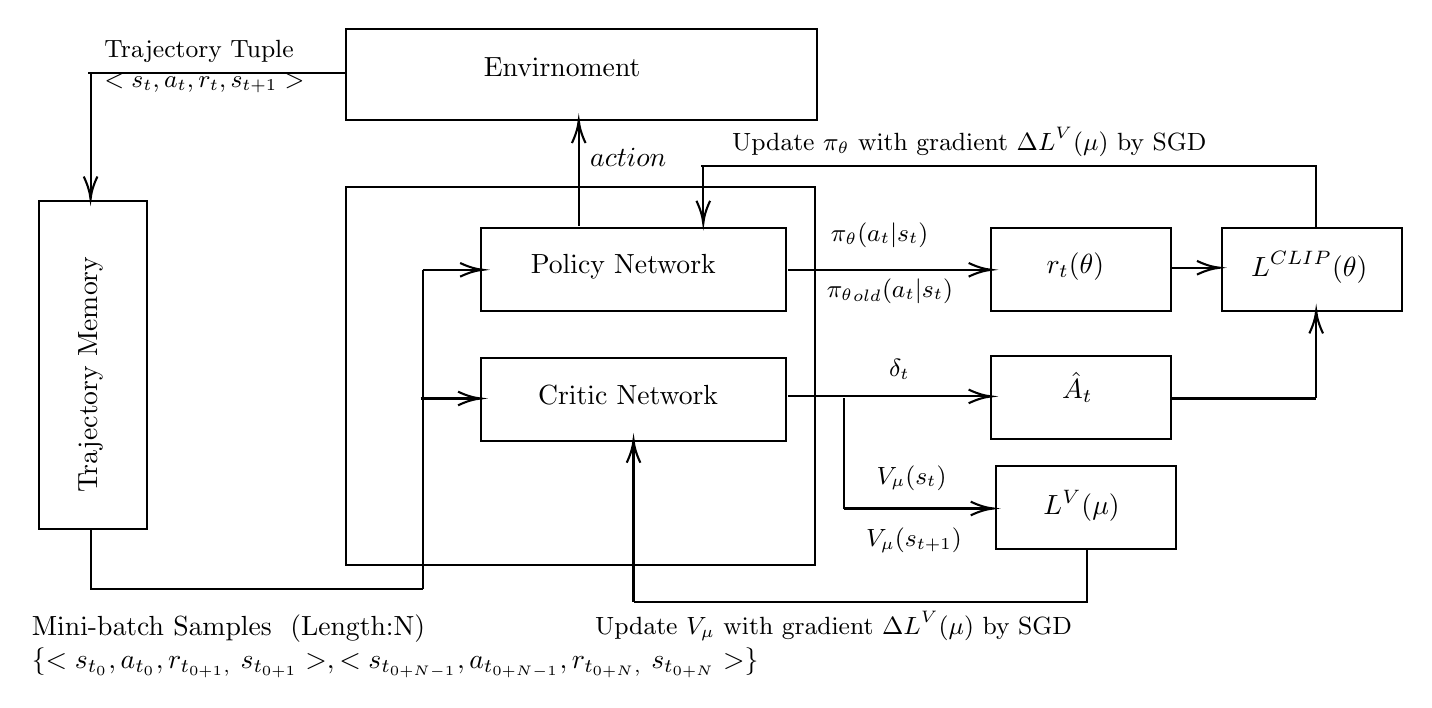
\begin{tikzpicture}[x=0.75pt,y=0.75pt,yscale=-1,xscale=1]
%uncomment if require: \path (0,338); %set diagram left start at 0, and has height of 338

%Shape: Rectangle [id:dp9978943115484824] 
\draw   (26.8,246.3) -- (26.8,88.3) -- (78.8,88.3) -- (78.8,246.3) -- cycle ;

%Shape: Rectangle [id:dp05267034608632715] 
\draw   (174.8,5.14) -- (401.8,5.14) -- (401.8,49.3) -- (174.8,49.3) -- cycle ;
%Shape: Rectangle [id:dp04578612721398789] 
\draw   (174.8,81.3) -- (400.8,81.3) -- (400.8,263.3) -- (174.8,263.3) -- cycle ;
%Shape: Rectangle [id:dp479111495997272] 
\draw   (240,101) -- (386.8,101) -- (386.8,141) -- (240,141) -- cycle ;

%Shape: Rectangle [id:dp3592684590066768] 
\draw   (240,164) -- (386.8,164) -- (386.8,204) -- (240,204) -- cycle ;

%Shape: Rectangle [id:dp5726876145364976] 
\draw   (485.5,101) -- (572.3,101) -- (572.3,141) -- (485.5,141) -- cycle ;

%Shape: Rectangle [id:dp8126568031433179] 
\draw   (597,101) -- (683.8,101) -- (683.8,141) -- (597,141) -- cycle ;

%Shape: Rectangle [id:dp24057721244799102] 
\draw   (488,216) -- (574.8,216) -- (574.8,256) -- (488,256) -- cycle ;

%Shape: Rectangle [id:dp21651348351379074] 
\draw   (485.5,163) -- (572.3,163) -- (572.3,203) -- (485.5,203) -- cycle ;

%Straight Lines [id:da2065459425933598] 
\draw    (313.4,281.3) -- (313.4,205.3) ;
\draw [shift={(313.4,203.3)}, rotate = 450] [color={rgb, 255:red, 0; green, 0; blue, 0 }  ][line width=0.75]    (10.93,-3.29) .. controls (6.95,-1.4) and (3.31,-0.3) .. (0,0) .. controls (3.31,0.3) and (6.95,1.4) .. (10.93,3.29)   ;
%Straight Lines [id:da5843246843678724] 
\draw    (387.8,182.3) -- (483.8,182.3) ;
\draw [shift={(485.8,182.3)}, rotate = 180] [color={rgb, 255:red, 0; green, 0; blue, 0 }  ][line width=0.75]    (10.93,-3.29) .. controls (6.95,-1.4) and (3.31,-0.3) .. (0,0) .. controls (3.31,0.3) and (6.95,1.4) .. (10.93,3.29)   ;
%Straight Lines [id:da5820279370707651] 
\draw    (387.8,121.3) -- (483.8,121.3) ;
\draw [shift={(485.8,121.3)}, rotate = 180] [color={rgb, 255:red, 0; green, 0; blue, 0 }  ][line width=0.75]    (10.93,-3.29) .. controls (6.95,-1.4) and (3.31,-0.3) .. (0,0) .. controls (3.31,0.3) and (6.95,1.4) .. (10.93,3.29)   ;
%Straight Lines [id:da03477812258414015] 
\draw    (414.8,236.3) -- (484.8,236.3) ;
\draw [shift={(486.8,236.3)}, rotate = 180] [color={rgb, 255:red, 0; green, 0; blue, 0 }  ][line width=0.75]    (10.93,-3.29) .. controls (6.95,-1.4) and (3.31,-0.3) .. (0,0) .. controls (3.31,0.3) and (6.95,1.4) .. (10.93,3.29)   ;
%Straight Lines [id:da09026891505962009] 
\draw    (414.8,183.3) -- (414.8,236.3) ;
%Shape: Right Angle [id:dp09688091613107686] 
\draw   (531.8,256) -- (531.8,281.3) -- (313.4,281.3) ;
%Straight Lines [id:da10002566422487891] 
\draw    (51.8,26.3) -- (51.8,85.3) ;
\draw [shift={(51.8,87.3)}, rotate = 270] [color={rgb, 255:red, 0; green, 0; blue, 0 }  ][line width=0.75]    (10.93,-3.29) .. controls (6.95,-1.4) and (3.31,-0.3) .. (0,0) .. controls (3.31,0.3) and (6.95,1.4) .. (10.93,3.29)   ;
%Straight Lines [id:da14348663665795947] 
\draw    (210.8,183.3) -- (237.8,183.3) ;
\draw [shift={(239.8,183.3)}, rotate = 180] [color={rgb, 255:red, 0; green, 0; blue, 0 }  ][line width=0.75]    (10.93,-3.29) .. controls (6.95,-1.4) and (3.31,-0.3) .. (0,0) .. controls (3.31,0.3) and (6.95,1.4) .. (10.93,3.29)   ;
%Straight Lines [id:da1581117014190938] 
\draw    (211.8,121.3) -- (238.8,121.3) ;
\draw [shift={(240.8,121.3)}, rotate = 180] [color={rgb, 255:red, 0; green, 0; blue, 0 }  ][line width=0.75]    (10.93,-3.29) .. controls (6.95,-1.4) and (3.31,-0.3) .. (0,0) .. controls (3.31,0.3) and (6.95,1.4) .. (10.93,3.29)   ;
%Straight Lines [id:da3327122153372011] 
\draw    (211.8,121.3) -- (211.8,275.3) ;
%Shape: Right Angle [id:dp7457457500271234] 
\draw   (211.8,275.3) -- (51.8,275.3) -- (51.8,246) ;
%Straight Lines [id:da24558256059318717] 
\draw    (174.8,26.3) -- (50.8,26.3) ;
%Straight Lines [id:da1907077659365608] 
\draw    (287,100) -- (287,51.3) ;
\draw [shift={(287,49.3)}, rotate = 450] [color={rgb, 255:red, 0; green, 0; blue, 0 }  ][line width=0.75]    (10.93,-3.29) .. controls (6.95,-1.4) and (3.31,-0.3) .. (0,0) .. controls (3.31,0.3) and (6.95,1.4) .. (10.93,3.29)   ;
%Straight Lines [id:da25181356746653694] 
\draw    (347,71.3) -- (347,97) ;
\draw [shift={(347,99)}, rotate = 270] [color={rgb, 255:red, 0; green, 0; blue, 0 }  ][line width=0.75]    (10.93,-3.29) .. controls (6.95,-1.4) and (3.31,-0.3) .. (0,0) .. controls (3.31,0.3) and (6.95,1.4) .. (10.93,3.29)   ;
%Shape: Right Angle [id:dp9296457308111634] 
\draw   (345.8,71.3) -- (642.3,71.3) -- (642.3,101) ;
%Straight Lines [id:da7729636916978786] 
\draw    (642.3,183.3) -- (642.3,143) ;
\draw [shift={(642.3,141)}, rotate = 450] [color={rgb, 255:red, 0; green, 0; blue, 0 }  ][line width=0.75]    (10.93,-3.29) .. controls (6.95,-1.4) and (3.31,-0.3) .. (0,0) .. controls (3.31,0.3) and (6.95,1.4) .. (10.93,3.29)   ;
%Straight Lines [id:da8163897958062174] 
\draw    (572.8,183.3) -- (642.3,183.3) ;
%Straight Lines [id:da9600198123912971] 
\draw    (572.8,120.3) -- (593.8,120.3) ;
\draw [shift={(595.8,120.3)}, rotate = 180] [color={rgb, 255:red, 0; green, 0; blue, 0 }  ][line width=0.75]    (10.93,-3.29) .. controls (6.95,-1.4) and (3.31,-0.3) .. (0,0) .. controls (3.31,0.3) and (6.95,1.4) .. (10.93,3.29)   ;


% Text Node
\draw (44.3,230.3) node [anchor=north west][inner sep=0.75pt]  [rotate=-270] [align=left] {Trajectory Memory};
% Text Node
\draw (509.4,226) node [anchor=north west][inner sep=0.75pt]   [align=left] {$\displaystyle L^{V}( \mu )$};
% Text Node
\draw (518.4,169) node [anchor=north west][inner sep=0.75pt]   [align=left] {$\displaystyle \hat{A}_{t}$};
% Text Node
\draw (510.9,111.5) node [anchor=north west][inner sep=0.75pt]   [align=left] {$\displaystyle r_{t}( \theta )$};
% Text Node
\draw (609.4,111) node [anchor=north west][inner sep=0.75pt]   [align=left] {$\displaystyle L^{CLIP}( \theta )$};
% Text Node
\draw (265.9,175.5) node [anchor=north west][inner sep=0.75pt]   [align=left] {Critic Network};
% Text Node
\draw (262.4,112.5) node [anchor=north west][inner sep=0.75pt]   [align=left] {Policy Network};
% Text Node
\draw (239.8,17.65) node [anchor=north west][inner sep=0.75pt]   [align=left] {Envirnoment};
% Text Node
\draw (407,97) node [anchor=north west][inner sep=0.75pt]  [font=\small] [align=left] {$\displaystyle \pi _{\theta }( a_{t} |s_{t})$};
% Text Node
\draw (405,124) node [anchor=north west][inner sep=0.75pt]  [font=\small] [align=left] {$\displaystyle {\pi _{\theta }}_{old}( a_{t} |s_{t})$};
% Text Node
\draw (435,163) node [anchor=north west][inner sep=0.75pt]  [font=\small] [align=left] {$\displaystyle \delta _{t}$};
% Text Node
\draw (429,214) node [anchor=north west][inner sep=0.75pt]  [font=\small] [align=left] {$\displaystyle V_{\mu }( s_{t})$};
% Text Node
\draw (424,244) node [anchor=north west][inner sep=0.75pt]  [font=\small] [align=left] {$\displaystyle V_{\mu }( s_{t+1})$};
% Text Node
\draw (57,9) node [anchor=north west][inner sep=0.75pt]  [font=\small] [align=left] {Trajectory Tuple\\$\displaystyle < s_{t} ,a_{t} ,r_{t} ,s_{t+1}  >$};
% Text Node
\draw (22,286) node [anchor=north west][inner sep=0.75pt]   [align=left] {Mini-batch Samples \ (Length:N)\\$\displaystyle \{< s_{t_{0}} ,a_{t_{0}} ,r_{t_{0+1} ,\ } s_{t_{0+1}}  >,\dotsc < s_{t_{0+N-1}} ,a_{t_{0+N-1}} ,r_{t_{0+N} ,\ } s_{t_{0+N}}  >\}$};
% Text Node
\draw (293.4,284.3) node [anchor=north west][inner sep=0.75pt]  [font=\small] [align=left] {Update $\displaystyle V_{\mu }$ with gradient $\displaystyle \Delta L^{V}( \mu )$ by SGD};
% Text Node
\draw (359.4,51) node [anchor=north west][inner sep=0.75pt]  [font=\small] [align=left] {Update $\displaystyle \pi _{\theta }$ with gradient $\displaystyle \Delta L^{V}( \mu )$ by SGD};
% Text Node
\draw (291,61.3) node [anchor=north west][inner sep=0.75pt]   [align=left] {$\displaystyle action$};


\end{tikzpicture}}
    \caption{Flowchart of actor critic based PPO learning model \cite{LimHun_ppo_flowchart}}
    \label{fig:ppo_flowchart}
\end{figure}

\begin{table}[H]
\centering
        
\begin{tabular}{p{0.75\textwidth}|p{0.1\textwidth}}
\toprule
 Hyper-parameter & Value \\
\midrule
 Clipping parameter ($\displaystyle \epsilon $) & 0.2 \\
\hline 
 Optimization algorithm & Adam \\
\hline 
 Learning rate ($\displaystyle \eta _{\mu } ,\eta _{\theta }$) & 0.0001 \\
\hline 
 Discount factor ($\displaystyle \gamma $) & 0.99 \\
\hline 
 The number of steps to run for each environment per update & 1000 \\
\hline 
 Entropy coefficient for the loss calculation & 0.01 \\
\hline 
 Number of training mini batches per update & 4 \\
 \bottomrule
\end{tabular}
\caption{PPO Algorithm Hyper-parameter configuration}
\label{tbl_hyperparam_PPO}
\end{table}

\noindent After pre training, model is trained for $16 \cdotp 10^6$ time steps with 1000 steps per episode using PPO algorithm. \autoref{fig:PPO_LOG_16M} shows reward per episode and rolling average. Notice how model learned within 5000 episodes, and later reward is saturated within 500 to 600.
\begin{figure}[H]
    \centering
    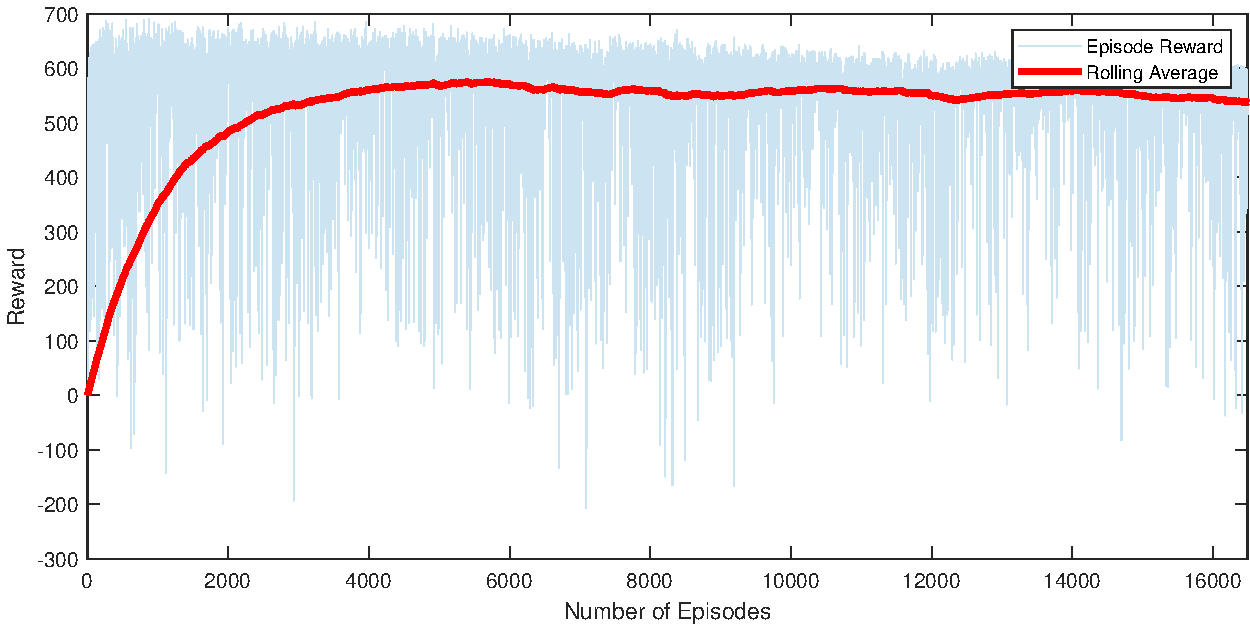
\includegraphics[width=\textwidth]{figures/plots/RL/PPOlog16M.pdf}
    \caption{Averaged episode reward for 16000 episodes of PPO training}
    \label{fig:PPO_LOG_16M}
\end{figure}
\subsection{Test Results}
Let us consider a test case, Neural Network based steering has to cancel attitude error in terms of Euler angles $\displaystyle \phi ,\theta ,\psi =[ -179\ ,\ -37,\ \ 140] \ \deg$ considering initial and final state shown in \autoref{tbl:nn_vscmg_states}
\begin{table}[H]
        \centering
        
\begin{tabular}{p{0.16\textwidth}|p{0.50\textwidth}|p{0.2\textwidth}}
\toprule 
 Parameter & Value & Unit \\
\midrule 
 $\displaystyle q$ & $\displaystyle [ 0.3036\ \ \ \ 0.3228\ \ \ -0.8891\ \ \ -0.1146]^{T}$ & - \\
\hline 
 $\displaystyle \omega $ & $\displaystyle [ 0\ 0\ 0]^{T}$ & $\displaystyle \deg /\sec$ \\
\hline 
 $\displaystyle q_{d}$ & $\displaystyle [ 1\ 0\ 0\ 0]^{T}$ & - \\
\hline 
 $\displaystyle \omega _{d}$ & $\displaystyle [ 0\ 0\ 0]^{T}$ & $\displaystyle rad/\sec$ \\
\hline 
 $\displaystyle \delta $ & $\displaystyle [ -0.7729\ \ \ \ 1.2424\ \ \ \ 0.6058\ \ \ \ 2.6412]^{T}$ & $\displaystyle rad$ \\
\hline 
 $\displaystyle \Omega $ & $\displaystyle [ 0\ 0\ 0\ 0]^{T}$ & $\displaystyle rad/\sec$ \\
 \bottomrule
\end{tabular}
        \caption{Initial and desired states for Attitude error tracking with Neural Network based VSCMG steering Law }
        \label{tbl:nn_vscmg_states}
        \end{table}
\noindent Results of error canceling maneuver using Neural network based steering are in \autoref{fig:nn__Torque_1} to \autoref{fig:nn__Omega_dot}. Being long slew maneuver, initial attitude error was large as consequence large demand torque variation can seen in first few seconds although after 10 seconds.
\begin{figure}[H]
    \centering
    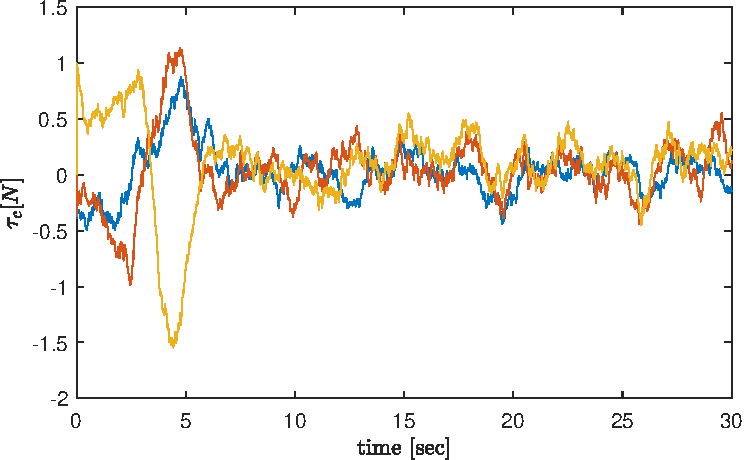
\includegraphics[width=\textwidth]{figures/plots/RL/nn_Torque.pdf}
    \caption{NN based steering: Required torques}
    \label{fig:nn__Torque_1}
\end{figure}
\noindent Variations in reaction wheels spins are more than that compared to gimbal angles, hence we can infer neural network has prioritized RWs over CMGs for this maneuver.
\begin{figure}[H]
    \centering
    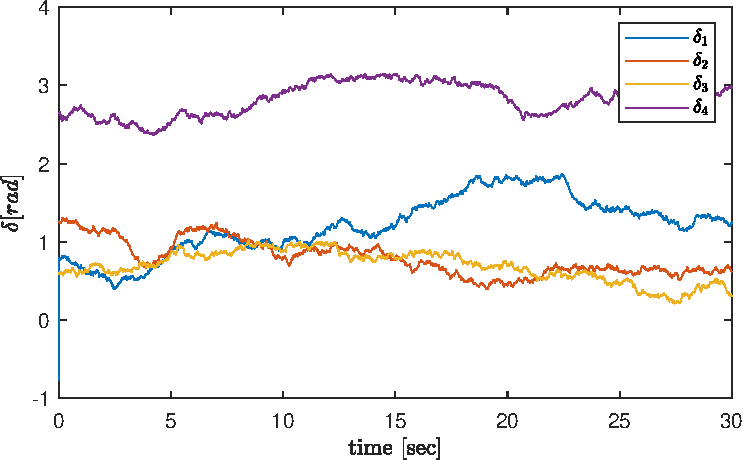
\includegraphics[width=\textwidth]{figures/plots/RL/nn_delta.pdf}
    \caption{NN based steering: Gimbal angles}
    \label{fig:nn__delta}
\end{figure}
\begin{figure}[H]
    \centering
    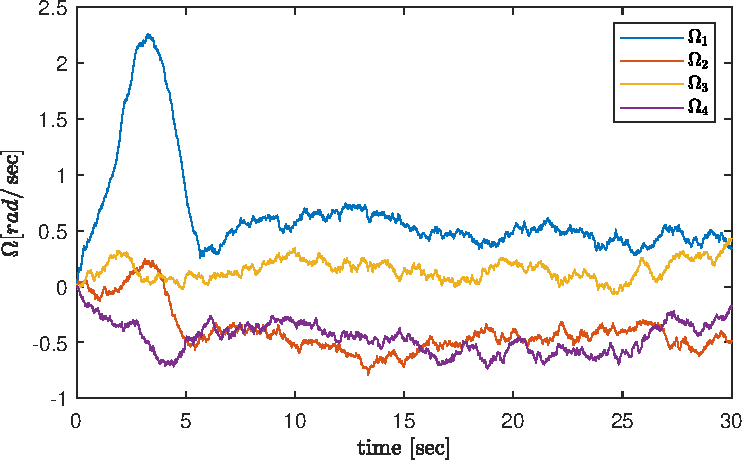
\includegraphics[width=\textwidth]{figures/plots/RL/nn_Omega.pdf}
    \caption{NN based steering: RW velocities}
    \label{fig:nn__Omega}
\end{figure}

\begin{figure}[H]
    \centering
    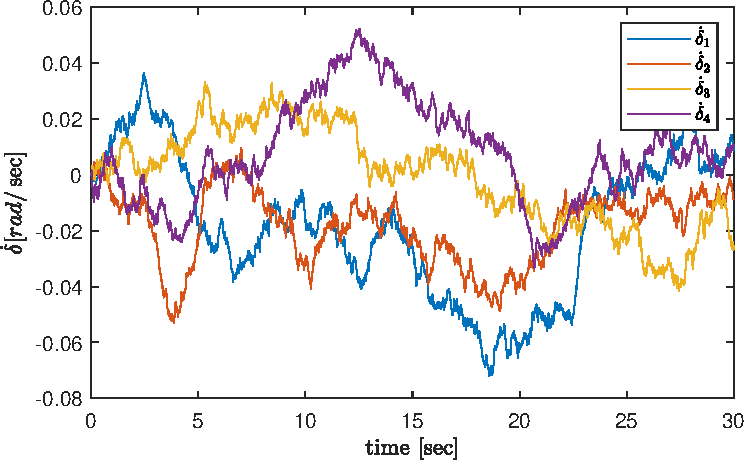
\includegraphics[width=\textwidth]{figures/plots/RL/nn_Delta_dot.pdf}
    \caption{NN based steering: Gimbal Velocities}
    \label{fig:nn__Delta_dot}
\end{figure}
\noindent \autoref{fig:nn__Delta_dot} and \autoref{fig:nn__Omega_dot} are control action performed by agent. Notice order of magnitude of RW accelerations and gimbal velocities are within permissible range and no large variation occurred.
\begin{figure}[H]
    \centering
    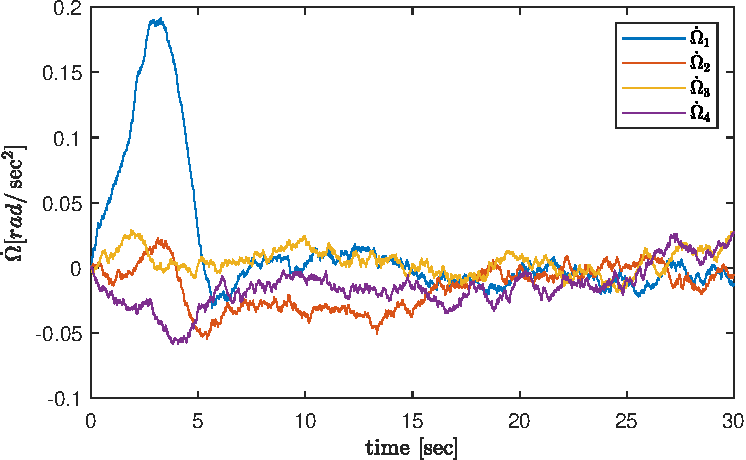
\includegraphics[width=\textwidth]{figures/plots/RL/nn_Omega_dot.pdf}
    \caption{NN based steering: RW Accerlations}
    \label{fig:nn__Omega_dot}
\end{figure}
\noindent Output data of neural network can be amplified or attenuated based on steady state requirements, moreover different activation functions at output layer can be used. A GUI based script is developed in order to monitor states and 3d visualization of VSCMG. Screenshot of testing trained PPO model is shown in \autoref{fig:model_explorer}. Main advantage of script is along with plots, attitude command and other model related parameters can be updated in real time, giving user an option for better calibrating the ACS according to required performance. 
\begin{figure}[H]
    \centering
    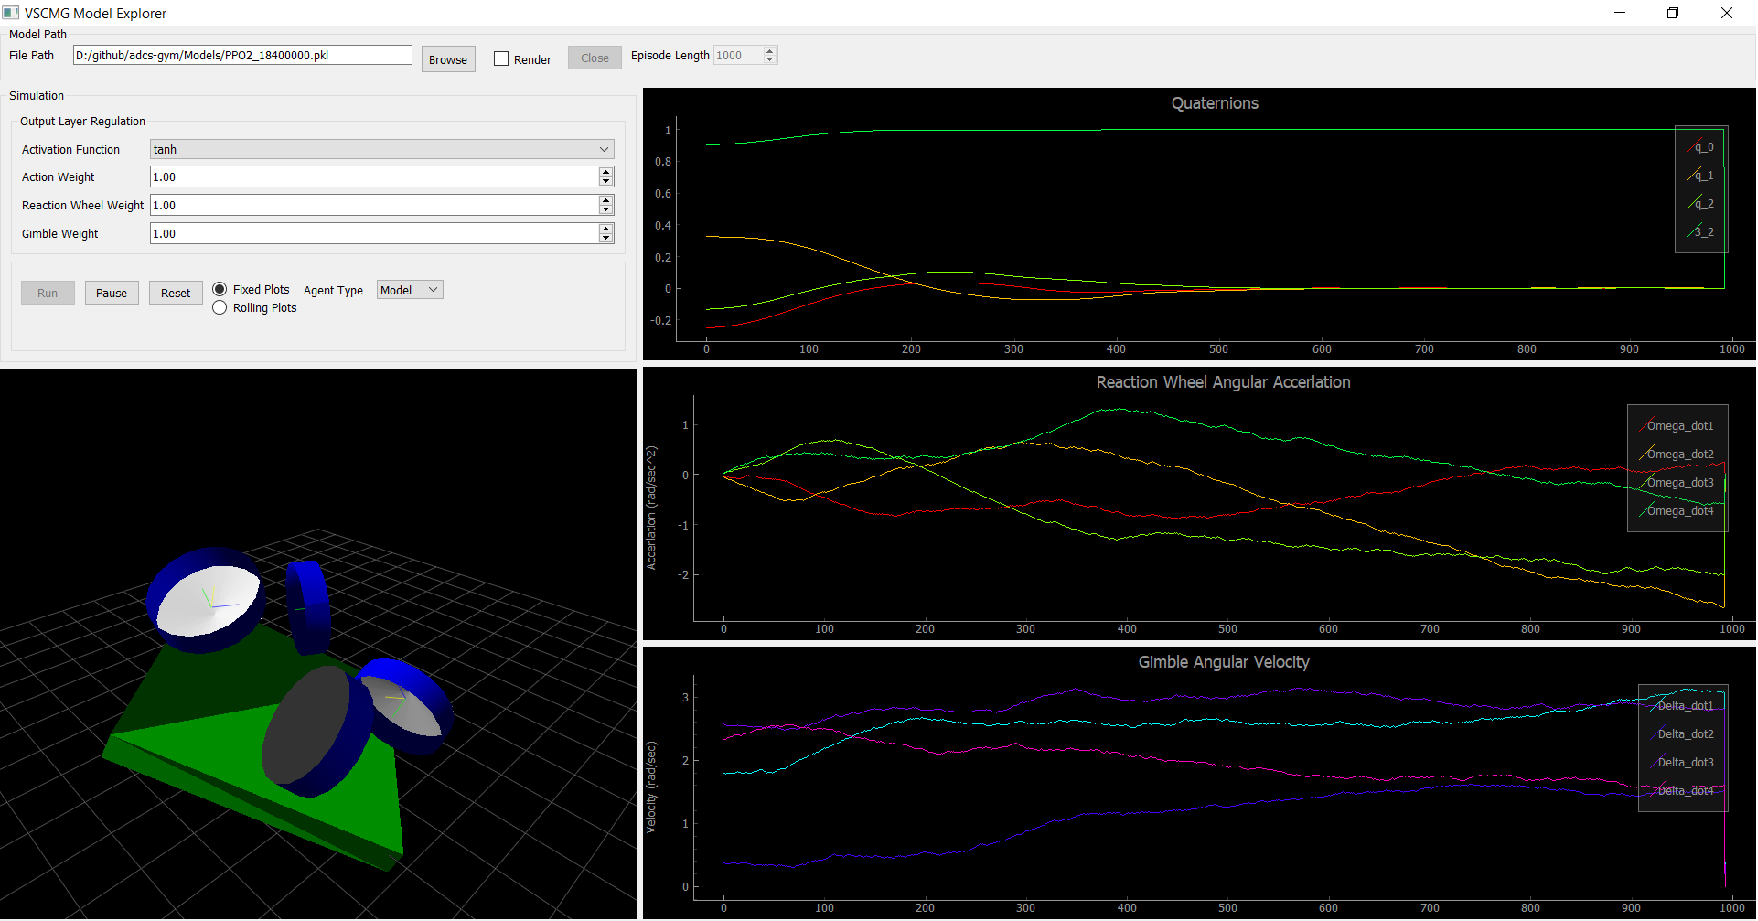
\includegraphics[width=\textwidth]{figures/AI/ModelExplorer1.pdf}
    \caption{VSCMG Model and expert agent Testing GUI}
    \label{fig:model_explorer}
\end{figure}


\section{Comparison of Neural Network and SR-VSCMG Steering Law}
\newacronym{sr-vscmg}{SR-VSCMG}{Singularity-Robust VSCMG Steering Law}
Following discussion assumes regulation maneuver with initial attitude error of $90^\circ$ in yaw angle has to be canceled. In order to evaluate the performance of steering law, spacecraft actuators are deliberately kept in singular states as shown in  \autoref{tbl:nnvscmg_params}. Notice angular momentum of all reaction wheels is zero, moreover required torque is orthogonal to CMG torque axis. 
\begin{table}[ht]
        \centering
\begin{tabular}{|p{0.2\textwidth}|p{0.4\textwidth}|p{0.3\textwidth}|}
\hline 
 Parameter & Value & Unit \\
\hline 
 $\displaystyle q$ & $\displaystyle [ 1\ 0\ 0\ 0]^{T}$ & - \\
\hline 
 $\displaystyle q_{d}$ & $\displaystyle [ 0.7071\ 0\ 0\ 0.7071]$ & - \\
\hline 
 $\displaystyle \omega _{d}$ & $\displaystyle [ 0\ 0\ 0]^{T}$ & $\displaystyle rad/\sec$ \\
\hline 
 $\displaystyle \delta $ & $\displaystyle [ 0,\ 0,\ 0,0]^{T}$ & $\displaystyle rad$ \\
\hline 
 $\displaystyle \Omega $ & $\displaystyle [ 0,\ 0,\ 0,\ 0]^{T}$ & $\displaystyle rad/\sec$ \\
\hline 
 $\displaystyle K_{w}$ & 4.4 & - \\
\hline 
 $\displaystyle K_{q}$ & 10.1 & - \\
 \hline
\end{tabular}
        \caption{Simulation parameters for regulation maneuver in order to cancel attitude error of $\displaystyle 90^{\circ }$ in yaw angle.}
        \label{tbl:nnvscmg_params}
        \end{table}
        
\noindent Results of Neural Network based and \acrfull{sr-vscmg} are concurrently simulated using specially developed Model Explorer software \autoref{fig:model_explorer} discussed in earlier section. Quaternions of simulation with neural network based steering are shown in \autoref{fig:nn_q} and \acrlong{sr-vscmg} shown in \autoref{fig:vs_q}. Notice that with NN based steering quickly approaches desired state within 5 seconds but a small steady state error persists, whereas with \acrshort{sr-vscmg} steering, slight overshoot is seen followed by long period osculation near desired state. Notice that with same control gains NN based steering quickly stabilizes and follows different trajectory than \acrshort{sr-vscmg} steering law. As shown in \autoref{fig:nnvscmg_w} small variation in body rates are visible in other two axis since NN based steering is following slightly different trajectory than SR-VSCMG for which variation in body rate is only along yaw axis. Even after approaching close to desired state small but significant amount of variations are persistent in all three body rates.
\begin{figure}[ht]
     \centering
     \begin{subfigure}[b]{0.49\textwidth}
         \centering
         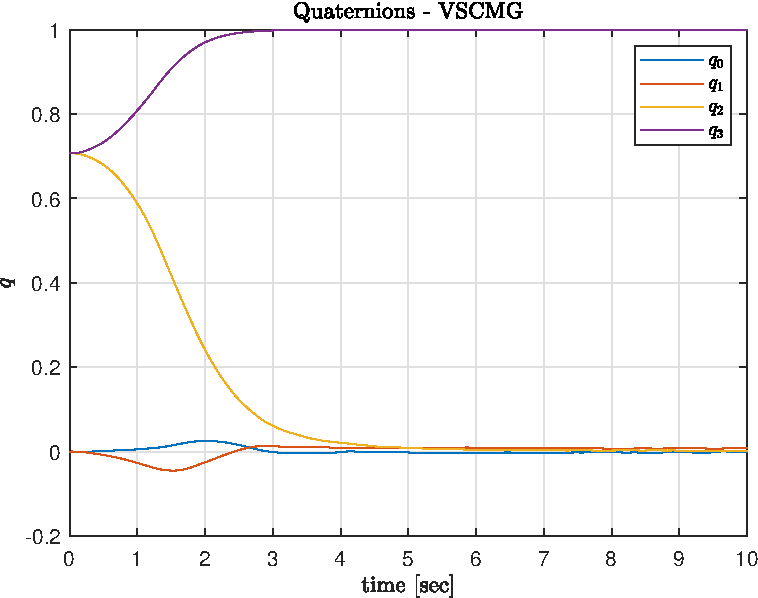
\includegraphics[width=\textwidth]{figures/plots/Results/vs-nn-q.pdf}
         \caption{}
         \label{fig:nn_q}
     \end{subfigure}
     \begin{subfigure}[b]{0.49\textwidth}
         \centering
         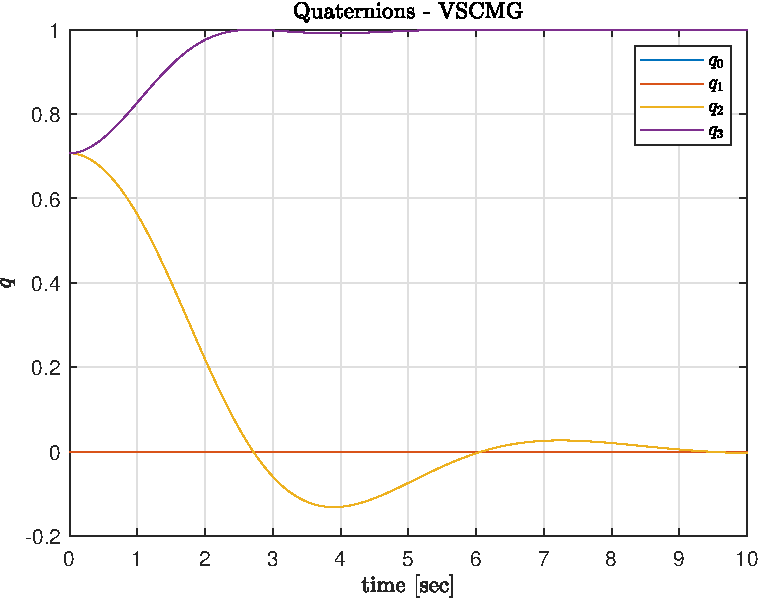
\includegraphics[width=\textwidth]{figures/plots/Results/vs-vs-q.pdf}
         \caption{}
         \label{fig:vs_q}
     \end{subfigure}
        \caption{Attitude quaternions : (a) Neural Network based steering (b) SR-VSCMG steering}
        \label{fig:nnvscmg_q}
\end{figure}

\begin{figure}[ht]
     \centering
     \begin{subfigure}[b]{0.49\textwidth}
         \centering
         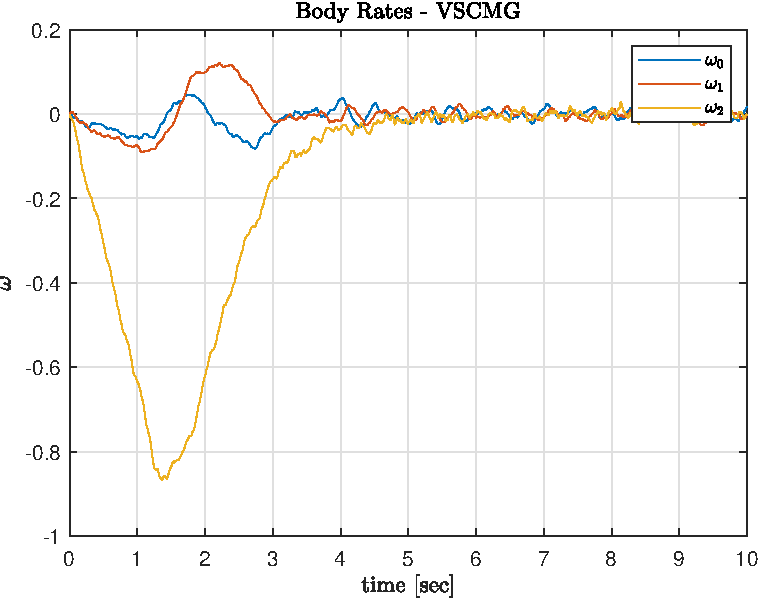
\includegraphics[width=\textwidth]{figures/plots/Results/vs-nn-w.pdf}
         \label{fig:nn_w}
     \end{subfigure}
     \begin{subfigure}[b]{0.49\textwidth}
         \centering
         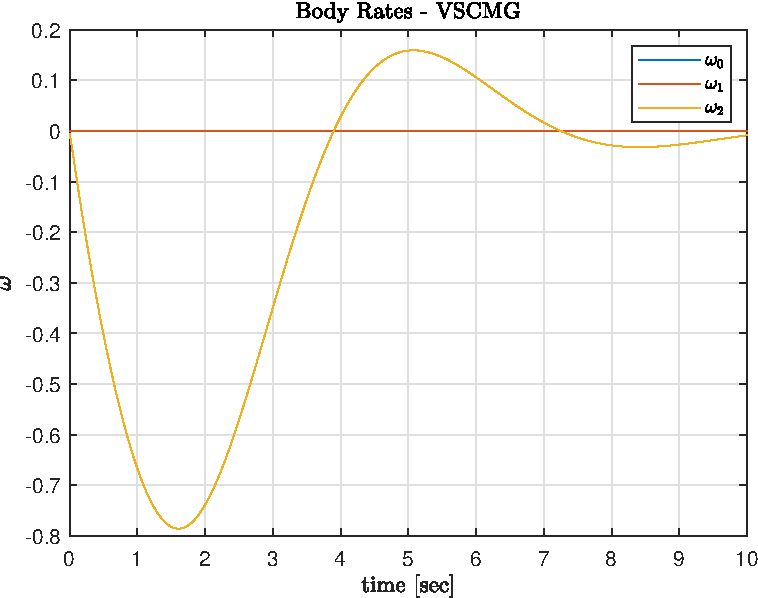
\includegraphics[width=\textwidth]{figures/plots/Results/vs-vs-w.pdf}
         \label{fig:vs_w}
     \end{subfigure}
        \caption{Body rates : (a) Neural Network based steering (b) SR-VSCMG steering}
        \label{fig:nnvscmg_w}
\end{figure}

\begin{figure}[ht]
     \centering
     \begin{subfigure}[b]{0.49\textwidth}
         \centering
         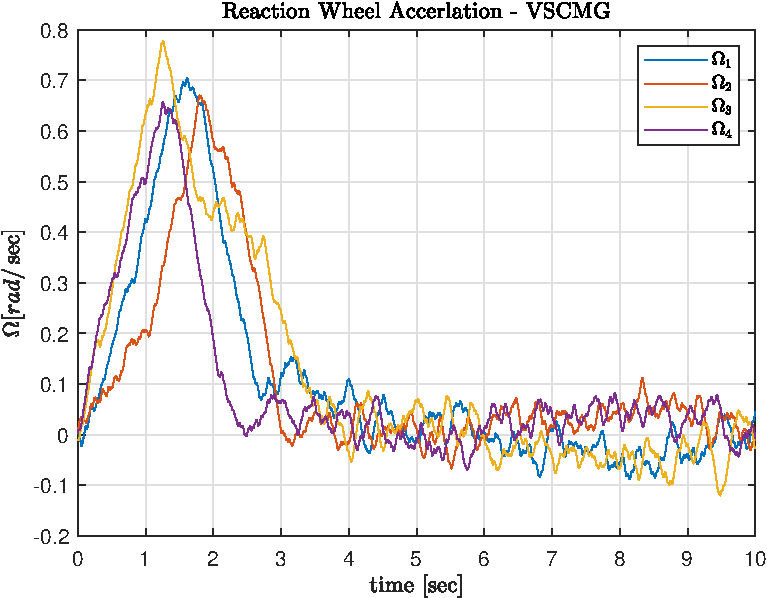
\includegraphics[width=\textwidth]{figures/plots/Results/vs-nn-Omg.pdf}
          \caption{}
         \label{fig:nn_Omg}
     \end{subfigure}
     \begin{subfigure}[b]{0.49\textwidth}
         \centering
         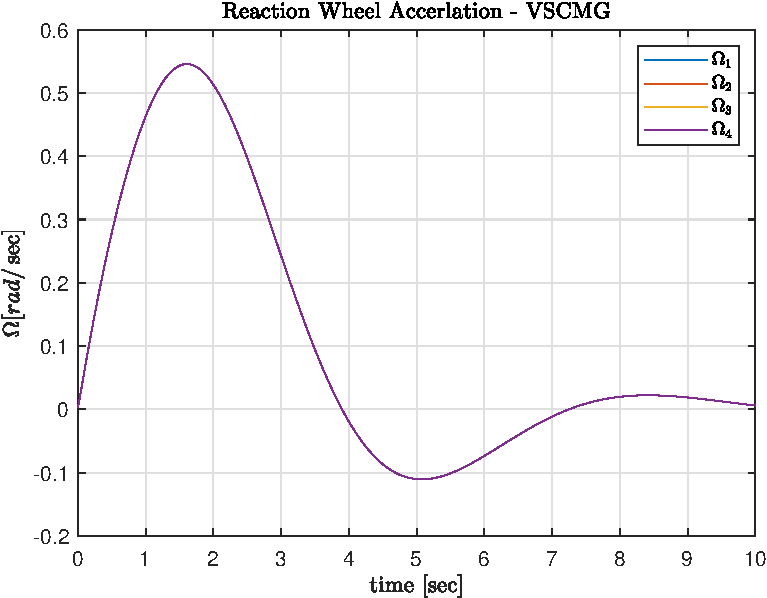
\includegraphics[width=\textwidth]{figures/plots/Results/vs-vs-Omg.pdf}
          \caption{}
         \label{fig:vs_Omg}
     \end{subfigure}
     
        \caption{Reaction wheel angular velocity : (a) Neural Network based steering (b) SR-VSCMG steering}
        \label{fig:nnvscmg_Omg}
\end{figure}


\noindent Each reaction wheel wheel is running at slightly different angular velocity in case of NN based steering, in fact this is the reason we can observe slightly different path followed than shortest path as in case of SR-VSCMG steering law in which only reaction wheel based control is followed throughout the maneuver. \autoref{fig:nnvscmg_sings} depicts three types of singularities. System becomes singular in case of rank deficiency that is transformation matrix is no longer full rank and hence non invertible. Degree or closeness to singularity can be measured with taking determinant of matrix. Here CMG singularity measure $m_c = \det(CC^T)$, Reaction wheel singularity measure measure $m_s = \det(DD^T)$ and complete VSCMG singularity measure measure $m_{vscmg} = \det(QQ^T)$ is shown in \autoref{fig:nnvscmg_sings}. CMGs are in singular state at the beginning since all reaction wheels are at rest. As angular momentum of RW is increased CMGs are getting away from singular state. Notice that in case of NN based steering distance from singularity is much higher at maximum RW angular momentum. Measure of RW remains constant in case of SR-VSCMG steering law since only RWs are used throughout the maneuver and gimbal angle remains constant. Whereas in case of NN-Steering, reaction wheel are moving far away from singularity due to variation in gimbal angle. Another contributing factor for increased in singular distance of RW singularity is different angular momentum of RWs.

\begin{figure}[ht]
     \centering
     \begin{subfigure}[b]{0.3\textwidth}
         \centering
         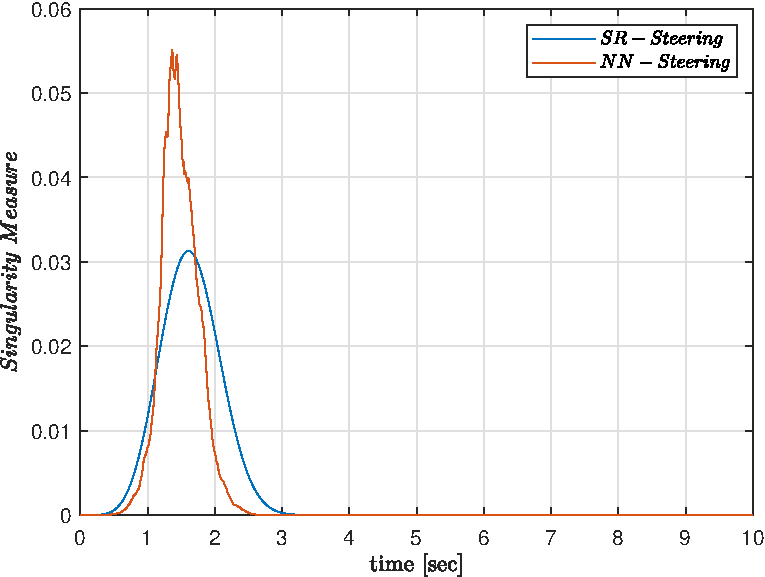
\includegraphics[width=\textwidth]{figures/plots/Results/vs-vs-CC.pdf}
        \caption{}
    \label{fig:nnvscmg_CC}
     \end{subfigure}
     \begin{subfigure}[b]{0.3\textwidth}
         \centering
         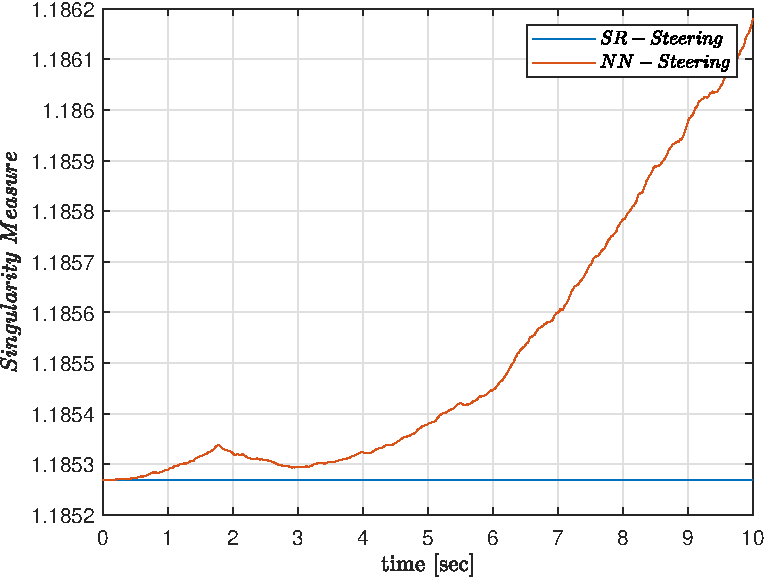
\includegraphics[width=\textwidth]{figures/plots/Results/vs-vs-DD.pdf}
          \caption{}
        \label{fig:nnvscmg_DD}
     \end{subfigure}
      \begin{subfigure}[b]{0.3\textwidth}
         \centering
         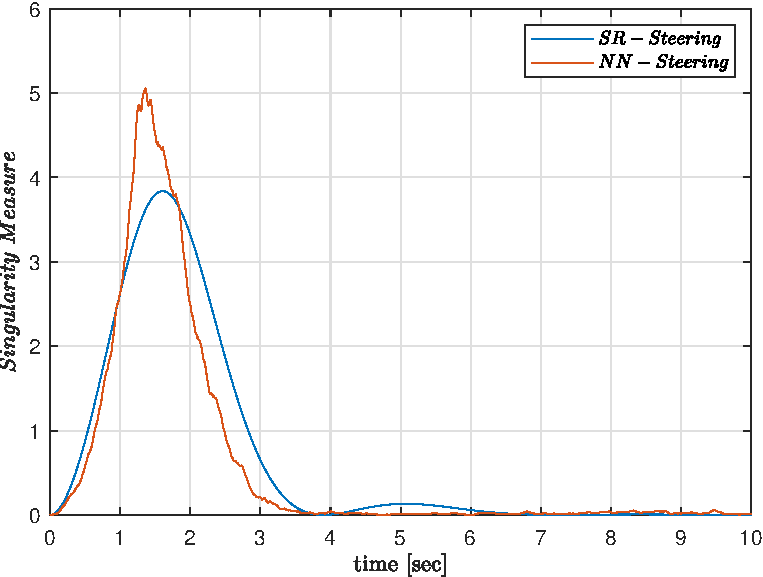
\includegraphics[width=\textwidth]{figures/plots/Results/vs-vs-QQ.pdf}
          \caption{}
        \label{fig:nnvscmg_QQ}
     \end{subfigure}
        \caption{System approaches singular state as singularity measure tends to zero (a) CMG singularity; (b) Reaction Wheel singularity and (c) VSCMG singularity}
        \label{fig:nnvscmg_sings}
\end{figure}

\begin{figure}[ht]
     \centering
     \begin{subfigure}[b]{0.49\textwidth}
         \centering
         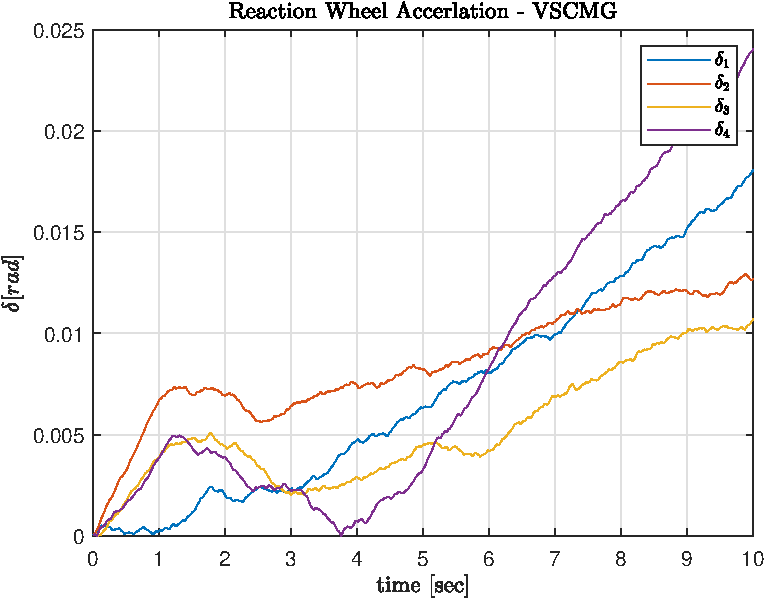
\includegraphics[width=\textwidth]{figures/plots/Results/vs-nn-delta.pdf}
          \caption{}
         \label{fig:nn_delta}
     \end{subfigure}
     \begin{subfigure}[b]{0.49\textwidth}
         \centering
         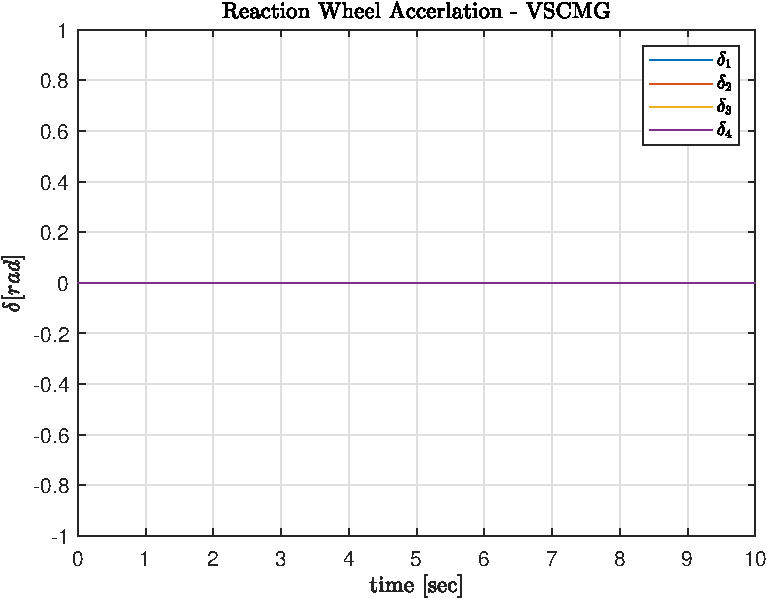
\includegraphics[width=\textwidth]{figures/plots/Results/vs-vs-delta.pdf}
          \caption{}
         \label{fig:vs_delta}
     \end{subfigure}
     
        \caption{CMG gimbal angles : (a) Neural Network based steering (b) SR-VSCMG steering}
        \label{fig:nnvscmg_delta}
\end{figure}

\noindent From above results it is clear that SR-VSCMG steering law provides more precise attitude tracking performance, although Neural network based steering is better at quickly approaching desires state following different trajectory with maintain body in  allowable range. NN based steering is inversion free technique thus very large velocities are not present in proximity of singularity. Steady state error and body rate oscillations in proximity of desired state can be reduced by regulating output layer by appropriate activation such as softmax and by filtering the output in order provide smooth actions to actuators. After numerous Monte Carlo simulations it is observed that NN based agent always converges to desired states but may follow trajectories which are not intuitive or similar to SR-VSCMG law. NN performance can be improved by more training and selecting better reward function crafted for required performance. A Hybrid of both steering law can be used, NN based steering for large slew maneuvers when error is large and SR-VSCMG based steering when current state is in proximity of desired state i.e. when error is small.